% Created 2021-06-22 Tue 23:39
% Intended LaTeX compiler: pdflatex
\documentclass[9pt, b5paper]{article}
\usepackage[UTF8]{ctex}
\usepackage{fontspec}
\usepackage{graphicx}
\usepackage{xcolor}
\usepackage{multirow}
\usepackage{multicol}
\usepackage{float}
\usepackage{textcomp}
\usepackage{geometry}
\geometry{left=1.2cm,right=1.2cm,top=1.5cm,bottom=1.2cm}
\usepackage{algorithm}
\usepackage{algorithmic}
\usepackage{latexsym}
\usepackage{natbib}
\usepackage{listings}
\usepackage{minted}
\usepackage[xetex,colorlinks=true,CJKbookmarks=true,linkcolor=blue,urlcolor=blue,menucolor=blue]{hyperref}
\author{deepwaterooo}
\date{\today}
\title{成长的故事 —— 我和表哥}
\hypersetup{
 pdfauthor={deepwaterooo},
 pdftitle={成长的故事 —— 我和表哥},
 pdfkeywords={},
 pdfsubject={},
 pdfcreator={Emacs 27.1 (Org mode 9.3)}, 
 pdflang={English}}
\begin{document}

\maketitle
\tableofcontents


\section{我最亲爱的表哥(4)}
\label{sec:org7af697e}

亲爱的表哥,生日快乐!

亲爱的表哥,这过去的数十年来,你一直都是我最想要嫁的人,是我今年秋天想要返回Pullman的土地上、返回WSU的校园里去读书、去读博士的源因、是我今年8月份离婚程序结束后、想要为其生儿育女、共同携手走完余生的人。

尽管我这个早年有着严重选择困难症的人现在的脑海里对各种信息的处理仍然显得万千纠结、不得要领,但我却清楚地知道自己心里的想法与愿望,只要亲爱的表哥你能够接受我,我随时都是准备好、都可以与你结婚、随时都准备好、都想要为你生儿育女的人!!!所以,请你不要放走我、不要再赶走我,我已经不再是当年的幼稚小孩,也不是你随便赶一赶、就会就能够被你违心地赶得走的,我真诚地想要与你走完余生!所以,也请你慎重考虑。

回想我的职场生涯,我终于还是觉得我就是被那个想要逼良为娼的三大中文职场圈死了职场人生的人(他们造就了一种势,把人圈死在里面,但实际上这个势是他们虚设的,它们的目的仅在于想要逼当事人去作娼奴性奴),回想这个踏上这片国士便几乎被注定的命运,心里仍会有很多的不满与不平,但只要最终我能够得到我亲爱的表哥你,我今生仍然开心知足,求仁得仁有何怨!

亲爱的表哥,就让我们互相执子之手、与子偕老,共同走完余生吧!

十年的磋砣岁月,不管我们是否真心愿意各自过成现在目前的这个样子,我们也都经历了太多。

我是觉得,在这个我几乎就快要丧失掉生育能力的青春的尾巴,如果我还要任由亲爱的表哥你将我一再地赶走,我们会miss掉太多的东西:会miss掉我们共同生儿育女、将它们抚养成人的机会、miss掉我们力所能及能够真正走到一起、生活到一起过幸福晚年的机会。这些,如果再如过去我很幼稚年代般miss掉十年,哪怕是晚年我们能够有几年光景还能呆在一起,仍然会是生命不能承受的遗憾,我会感到深深遗憾、承受不来!

如果在这个最重要的、我仅存的生育能力青春尾巴的关口,我还不回到亲爱的表哥你的身边,尽自己的最大努力把握住自己想要把握的今生唯一的幸福机会,我剩下的哪怕是还有几年光景也只怕是不得安生。所以,这个秋天,我想要回去,一定回去,回到亲爱的表哥你所在的Pullman的土地上,回到亲爱的表哥你所在的WSU的校园里去读书,让我们在同一座校园里,组建家庭、共同欢度余生。 

前面的专业职场生涯里的逼良为娼我已经写得很多了,大家都知晓;

后来的,非专业职场中的,前面也有力所能及地提及,一如现在他们想要逼我走向的两个不同的方向:如果我们能够顺从他们的逼迫,并有一定的专业能力与素养在专业职场生存,他们为想办法为这些被逼女性洗地洗白,再次最终分配到专业职场(而现在的压迫与追杀封杀是它们想要逼良为娼不得不采取的手段而已);如果我像他们最想要逼我走的easy str,去开个餐馆谋求生存,我的路是被他们毁得最惨的,君不见加州硅谷各餐饮的诸多老板娘都是他们逼良为娼的结果,而且餐馆老板娘因为作案风险低,存在一个老板娘为多职场高管或多幕后佬儿们侵战占的可能性。硅谷那些声音嘶哑的餐馆老板娘,看看想想便知。

我想我仍不至于绝望、不至于被他们逼至绝境,因为我始终都还有亲爱的表哥你,这个我最想要与之共度余生的人;前面去年2020年赌场里赢过的那一点儿钱与前几前我们输过的钱相比,少之又少,但也仅是他们想要逼良为娼的手段之一。我的历史始终都是清白的,他们拿我——这样一个被亲爱的表哥你培养树立了爱情信仰的人,是无能为力的、无从下口的,过去如此,现在如此,将来也会永远如此。

因为我的生活会move on,我会回到亲爱的表哥的身边,而他们也最终只能放弃这个被他们紧盯了十多年的目标,也让他们的这个黑色产业链最终真相大白于天下,在老百姓的心目中生根,相信也会只有越来越少的女性会陷入到他们的这种逼迫中去。 

亲爱的表哥,写到这里,我终于是完成了我们共同完成的一件壮举:破除三大中文网站逼良为娼的产业化操作,将他们如此炒作自家网红、并最终逼良为娼的黑色产业链彻底白菜化,让他们这一见不得光的暗箱操作彻底见光死、让他们的这个产业链在广大小市民、在老百姓心目中遍地开花、了然于胸、一见便知、心知肚明,让越来越少的女性、女留学生们陷入到我曾经所遭遇的这些困境中来!

亲爱的表哥,这件事情、在你(和舅舅)的发动、在我快速成长与无限配合下,我们终于是合作完成了一件壮举,我们做到了:为往事干杯,为我们自己干一杯!

到2021年这个春天,我终于明白,09年秋季学期、舅舅不早不晚在我统计专业的最后一个学期、为我从韩国搬回来的亲爱的表哥你,就是真真正正要表哥你来作我的坚强后盾来着!不是早年间12年表哥你亲手播打911后我在人间炼狱里自己反省出来的自已是寄生草寄生虫,舅舅帮我搬回来的就是真真正正、我内心里最想要的,我的矿世爱情和我今生的终身归属!

有一种感动——惊心动魄,有一种遭遇——万劫不复,当我们遭遇了爱情、追寻过梦想、历经了沧伤,当我们重新回到梦开始的地方、回到我们分开出发的起点,亲爱的表哥,你还在等我吗,你还可以接纳今天的我吗?

亲爱的表哥,你可以接纳现在的我吗?你是否也如我般曾经沧海?你的沧海里是否可以容下我的眼泪?

亲爱的表哥,我们——你和我,有一个十年之约,我会欣然前往赴约,你准备好了吗?

这一次,这个月底(还有几天到这个月的31号,我就出发开车返回亲爱的表哥你所在的Pullman的土地上),我要回到亲爱的表哥你所在的Pullman的土地上,申请回到亲爱的表哥你所在的WSU的校园里读博士研究生,我要作亲爱的表哥你房间里的女主人,我想要陪你一起、我们共同走完余生!

亲爱的表哥,这次,我再也不会再走丢,你也一定要等着我,等我回到你身边,不许再播打什么911,不许你逃跑\textasciitilde{}!!!

昨天是你毕业四周年的日子,恭喜你,恭喜我们\textasciitilde{}! 

毕业四年了,工作几年了。 

\textbf{亲爱的表哥,你准备好,准备好今年可以娶我了吗?!!!我等着!!!}

\textbf{备注:一点儿澄清吧:}

其实,对于最近几天的舆论炒作,我已经很无语了。自从2010年我被他们盯了几年后,从三大中文网站内部开始炒,炒作出如日中天的名气,到自2020年4月我从中国疫区返回后前后在instacart、doordash做事,他们——三大中文媒体终于是借助这难得的我在他们平台做事的机会对我一黑再黑,黑的结果,当然是:当他们想要帮你维护世外天仙般的名气的时候,他们做到了,封印了一个人的人生十年;当他们想要黑掉一个人想要对当年的所谓的网红逼良为娼的时候,他们想要黑,借助各种手段的黑、借助租住地鬼窝里的人的故意设计一黑再黑,当然最终结果是在他们想要逼的时候,他们是当然能够把那份当年的名气黑得掉渣黑成媒炭的,他们做到了。

被他们黑掉,也只是时间早晚的问题。我只是一个微弱的个人,当一个团体对一个个人施加舆论暴力的时候,作为没有任何、没有多少社会资源的个人,是很难自我保护的。

今天被他们黑掉的结局,一如当年炒作的时候他们便安排好了所有人的结局:我会被他们故意按上撒谎的罪名,但我清楚地知道我没有;几十年来,所有当年哪怕是被炒得如日中天的网红,最终也难逃如我今天般被他们所谓“社会性死亡”————把一个人的人品个性炒作成死结的结局!但天是蓝的,水是清的,我对亲爱的表哥的爱是真的,并不因为他们的炒作、或是黑掉而有丝毫的质疑。人的感情的状态那么多种,我与我表哥的爱情就是如星座里所说般纠结在时间空间里,当这个世界上我那一年那几天真正“遇见”表哥遭遇了爱情,我对爱情的执着坚持便是以我表哥的立场为立场,以他的标准来要求自己,我愿意为他坚持、因为他的存在我做不到随遇而安,社会舆论从来都是一个很stupid的东西,不被社会大众接受并不代表别人就撒谎了、并不代表别人就不真心爱着,有些情侣明明就是相爱着,但形似分离又如何?我爱上了一个这样的人,我愿意为自己的爱坚持与守候,那是我余生的选择,与三大中文所炒作的撒谎与不撒谎无关,撒谎与我的人生自高三之后再无任何相关。 

但会不会被他们逼成他们想要的角色,不是像他们像想要黑我就能黑得掉那么简单的、这并不是他们想要做就能做得到的。因为我亲爱的表哥在我相对还很细稚的年龄已经为我树立了强大的爱情信仰,作为一个为爱而生的狮子,他们三大中文几十年炒作网红逼良为娼的历史上,想要逼别人他们也会有失败的时候,像我便会成为一个例外,因为我在变强大,情感上精神上专业上各个方面,而我也会选择守候在我亲爱的表哥的身边,看着他生活得开心幸福我便知足了。

三大中文的历史上我先前我提到过的有个四岁女儿的离婚单身生物博士后老顿姐姐、以及个别几个外嫁的姐姐也曾总结过(我有机会读到过):三大中文逼的是心智脆弱的女性个体,我是有自己的脆弱面,但我有我亲爱的表哥为我树立的爱情信仰、这个世界上有我亲爱的表哥的存在,有与我表哥相处的这过去十年的沉淀与精神力量,有爱情力量、亲情力量的精神支撑,我便不致沦落红尘。而且,我有着神等级的专业, 这个神等级的专业会一再帮助自己一再变强大,摆脱他们的魔掌。

大家敬请放心。

\section{2013 Summer Intern暑假实习(9)—— 还原当年三大中文舆论炒作的起始状态、立意与三大中文上它们自己作出的结论预}
\label{sec:org5bbc5c1}

亲爱的读者,写到这里,我已经无心再继续写下去了。

不是写到这里,我无心再写下去了,而是(像我这样沉浸式思维会翻来复去地去想,有时候就会难免)觉得如果我亲爱的表哥不够喜欢我、无法喜欢和接纳我,我可以就没有信心和勇气再写下去了吧。 

我仍然相信我亲爱的表哥真心喜欢我的,并且为我的成长付出和牺牲了很多,但我亲爱的表哥在我这个从小自卑长大的小弱弱这里,我们缺少了三个词、8个字母,我表哥那么强大,我缺少一份绝对地确定。

在这一季站出来写的最开始,我还是非常相信我亲爱的表哥是真心喜欢我的,并且这一年、今年我们是会结婚、可以走到一起的。

就像我的舅舅多年以前曾经说过的神话,当三大中文对我一再地逼、想要逼我去当性奴,我的舅舅当年的神话都是支撑我战胜困难、绝不屈从的一个支撑:因为我亲爱的表哥与我本身就没有太多的物质欲望,有情饮水饱、我们可以简单地生活得很好!所以我可以其它一切事情都不管不顾,一心一意只要将这一件事情做好、把握住今生最大的幸福便是当下生活的一切!

今年3月30日,事隔六年之后(继2014年12月27日我这之前最后一次见到我表哥,又隔了六年多)当我再一次地踏上征途、回到那个给我留下深刻、无限记忆的家,我亲爱的表哥却再一次地播打了911. 我的舅舅、和我亲爱的表哥,这个911还要播打多久、到什么时候他们才能够放下这一剥夺穷人生存资源的法律冷血武器?!!!我与舅舅、我表哥的亲情联系又何时才能重新真正建立起来呢?  


当这里面(我亲爱的表哥与我的爱情、我的表哥3月30日仍然播打了一次911,我当然会等到8月底等到我的离婚程序彻底结束、等到我亲爱的表哥可以完全接纳我的那一天)有一丝的不太确定,我便仍然还有生存的压力,我今年也已经42岁了,我可以为了我亲爱的表哥、为了自己心目中的爱情信仰与信念,同我表哥一样脱离尘世地执着,我表哥不结婚我便也不再结婚、我仍然是任何时候都随时准备好、随时都可以与表哥结婚的状态!!!但我表哥有工作、可以把自己的事情做得很好;而我也还需要像我表哥目前一个人暂时也还可以生活得很好一样、我也还需要为了自己的生存努力挣钱谋得生存、并从自己的专业领域努力谋得一席生存之地。

所以,我也就无法像先前一样、每天投入量的时间,只为发一篇或许并无人关注的贴文。毕竟,我亲爱的表哥能够与我真正走到一起、真真切切、实实在在地生活在一起才是对我来说余生生活最好的选择与出路。否则,我过的、精神上都是极其悲惨、过的是其它人的生活,这是不管(三大中文所炒作起、掀起的)舆论的风如何刮,我都会坚守的自已的内心——如何不是我亲爱的表哥能够接纳我、如果不是同我亲爱的表哥结婚、我今生都不再结婚!如果万一实在今年还是不能同我表哥结婚,那我也要像我表哥学习、努力做到独善其身!

原本,比如我亲爱的表哥接起电话,我表哥对我多说几句话,我都会开心很久,都有很大的信心接着写下去、写完;但当我越来越找不到支撑、而我与我亲爱的表哥的联接与信任、被三大中文媒体一再反方向作用力平衡、被大表姐一再从中作梗的时候,我就还是会受到这些环境的影响而显得很难再坚持写下去了。 

但我还是会尽自己的最大努力把自己的思维逻辑和立场阐述清楚。所以,接下来的部分,如果我还在接着往下写、接着更新的话,就让我们来试图回归当年的、我所理解和了解到的所有的真相。

首先,我自己的个人立场最重要。我仍然会回pullman,但在我亲爱的表哥主动联系我(这个或许会很快发生,如果我亲爱的表哥这些年是真心真意喜欢我的话,恩我相信这一点儿,我表哥如果有他喜欢的人,这些年里一定是我!!!或许永远不会再发生,如果他确实从来就不曾真正喜欢过的话,但是这点儿我不相信、现在不相信:我不相信我表哥从来不曾喜欢过我,这话只是大表姐给我洗脑的话)之前,我不会再主动与这家人有任何联系了(为我自己的安全考虑——我不希望再收获来自于舅舅或者是表哥的任何911或者更甚一步的行动了)。我想回Pullman读书,是我自己厌倦了硅谷大城市的肮脏、喧嚣,与亲近宁静小城市和大自然的需求、和我自己心底一份坚守自己爱情的信念与执着,以及想要以后永远远离硅谷、争取能够在小城市、学术圈勉强生存的愿望与努力。

是有这个愿望,但六月份回去了大家都在放暑假(学校院系里的老师、工作人员们),我申请学校联系老师都不太方便,我觉得我可能还是在这个硅谷再多呆两个月,到八月头回去,立即联系老师,能够秋季上学最好,实习不能秋季上学可能会往后拖一个学期吧。不过我会尽最大努力(如果实在申请不到任何奖学金、或是实在录取不了)秋天回学校读书(秋天脑袋比较清醒一点儿)。这两个月(六月七月,因为这个月底我一定会搬家)我会尽量再挣些学费生活费用供接下来上学用。因为还有两个月才回我表哥所在的Pullman的话,那这两个月我还是会因为我亲爱的表哥、因为与我表哥之间的爱情信念信仰、以及我表哥学校的运动队运动精神支撑而接着往下写,写到有一天我实在、再也找不到任何动力、或是再也找不到任何爱情信仰或环境的支撑为止。但可能不是每天都能更新很多,就每天、或是两三天,能写一点儿出来就更新一点儿吧。

三大的黑:他们黑我的时候,一如当年他们会故意禁网,故意制造人民群众不敢发声的网络场景,他们会禁我的IP,并发动每次为期一天左右的可以合理猜测的对我集中火力的黑,比如拿我个性中的某些缺点来故意黑我、集中火力地故意黑我;不留余地地!

我先前的观点,还曾想过要不要从王夏华处要结婚彩礼呢?现在,那些彩礼什么的我都不再想了。求仁得仁,能够得到我表哥我就很知足了。只求我不负任何人,就可以了,用我的舅舅12年4月他当作新闻发布会上的观念信条来要求自己。

12年、08年夏天舅舅把我送到加州硅谷人间繁华地来体验大城市的繁华。十多年里,我终于是看透了大城市繁华背后的虚幻、对大城市终于是不再向往、没有留念、甚至想要远走离去、去避开它的喧嚣纷杂。

我想要离去,那我想要去哪里呢?当然是想去表哥的城市去生活呀!

当我厌倦了城市的喧嚣纷杂与浮躁,我想念菁菁校园的静谧沉静,我想要回到表哥的故乡、舅舅也喜欢的、表哥工作的校园坐落的大自然中去!

作为一个农村长大的孩子,我喜欢广袤的大自然,我喜欢雨过天晴的滋润清新,我喜欢雨后、夜幕降临下的青草味道;

小时候二姐带我们去叔叔家做客,我们一定会选择下雨天去,应该下雨天去叔叔用他的渔网打鱼会比较有渔获,而我就是那个喜欢跟着叔叔去广袤的大自然中去呼吸新鲜空气的、捡渔虾的小P孩;

小时候同爸爸出去打鱼的时候夜晚里夜幕降临露水落下、滋润清新的夜幕下的青草味道,这些青草味道、雨过天晴的滋润清新都已经深深地刻在了我的灵魂深处;

我喜欢大学时期武汉的梅雨季节的雨水,这些雨水滋养着我的灵魂(和12月7日的校园广场绘画展,艺术陶冶情操,我的心灵得到洗涤与滋养)

2005年夏秋、当实验室一定不再是我的选择,我选择了去山青水秀的广西养病,帮助自己早日从困难中摆脱出来;

2013年夏天我终于鼓足勇气去锻炼身体(去山林中hiking),我把自己锻炼得比较好,我也把自己工作时的精神状态调整得比较好。

大家也看见了,我对自己这个认得的舅舅的看法是一分为二的。

今年的3月13、14日那个周末,我开始读了自己当年、早年传记中的大部分内容,可以清楚地读出当年那个幼稚的自己。所以,就像我自己所能够感觉到的舅舅曾经给予过的暗示,今年的3月15日早上八点零几分,我终于是鼓足勇气、于11年11月给舅舅打过一个电话(那年我的爸爸出意外,电话里我问舅舅我可不可以与表哥结婚、哪怕先只把结婚证领了都行,舅舅说表哥的感情不到位)多年以后再打电话给我的舅舅,我播通了舅舅的电话。 

电话里我向舅舅对自己当年的幼稚行为道歉(比如11年5月底回去也回去了,不听舅舅到底怎么说,一回家看见地上的东西转头就走等幼稚行为,电话里我并没能对舅舅讲这些我所认知的道歉细节)。舅舅倒也没有计较。电话里我两次问及舅舅“我表哥呢?!!!”这些年里,唯有那个心心恋恋的表哥仍然是她心底最深的眷恋、是她战胜所有硅谷三大中文逼良为娼黑势力的源动力,舅舅只答说他不知道。那我也只能主动事后自己联系过我表哥。问及我想像当年的表哥一样读个博士学位,舅舅却要坚定地把我锁定在硅谷,答说我想读博士,我可以在加州硅谷读博士——这会让我一再去想,舅舅电话里说要我留在硅谷的目的是什么?08年舅舅开车护送陪我前往硅谷的路上,他不是对我一再重申他觉得小城市的生活比较安静静谧吗?更何况,回到小城市,回到我表哥所在的城市,老大不小的我亲爱的表哥和我两个人也才能真正走到一起、重新组建家庭life也才能够move on的呀?!

一方面舅舅说,他不知道我表哥到底在哪里;另一方面,舅舅又不免提及表哥,舅舅电话里在我面前表扬我表哥说我表哥“你表哥他很聪明、也很有报负!”我亲爱的表哥、这些年里,在我这里自然是极其聪明、又待我很好的强大存在、作为源动力、精神动力支撑了我这过去的这些年!那舅舅口中,我表哥的报负是什么呢?

这些年里,因爱我表哥生恨也罢,我恨过舅舅、狠狠地恨过舅舅(现在已经没有那么恨了)、对大表姐王夏华做过的很多事情不平衡过,但一如三大中文所了解到了,我亲爱的表哥在我这里,从来都是一个完美无缺的存在;他们都知道,我对别人对别的任何人有任何的看法,我从来不曾说过我表哥有任何的不好,因为我亲爱的表哥,待我从来都是极好的——那场深入骨髓、灵魂深处的遇见,又怎么可能是俗世里曾经将就的婚姻对象、比如会随便发泄他的怒气脾气会随便对他自己的女人下狠动手打人的前夫可以随便相提并论的?!!!

就像我先前所写到的,我这辈子,什么时候都是随时准备好、随时都可以与表哥结婚的状态!!!

所以,我一定要回到我表哥的身边,哪怕只是呆在我表哥所在的Pullman WSU校园里去读书、去读一个不是很热门,但仍然极有意义的专业!

\begin{center}

\includegraphics[width=.9\linewidth]{./pic/readme_20210516_102713.png}
\end{center}

如果我的表哥十年了还不结婚,那我以后也可以不再结婚,直到表哥先找到他的幸福为止!因为我表哥曾经待自己的好,我愿意用自己的余生作陪葬,一如我表哥先前曾守候过我的幸福,我愿意守候亲爱的表哥余生的幸福!!!

\begin{center}

\includegraphics[width=.9\linewidth]{./pic/readme_20210515_095559.png}
\end{center}

这里,我想,我更想表达的是,对于我来说那场深入骨髓的遇见,我亲爱的表哥这里我相信也是爱情的;但退一万步,如果我表哥是把它当友情处理的,我同样尊重表哥待我的好,一如那场遇见成为开在灵魂深处的花,静静绽放在无数个午夜梦回的夜里、绽放在寂莫生活的思恋里。哪怕是一场美好的回忆,也都将永远被珍藏!!!

我的舅舅自然是有着不同处理的,他十岁随二外公离家避开斗地主的斗争而逃走闯社会,他的社会阅历与认知、他的透彻都迫使他站出来、帮助有可能不善处理感情问题的表哥、有可能因为过于善良不忍心拒绝我的表哥摆脱来自于三大中文社会舆论压力与困扰——这个在2010年12月、2011年1月2月是客观存在的:因为当时三大的舆论炒作已经分为了两个方向:如果我表哥是真爱我,待我那般好,我与我表哥遇见的那场告别、我表哥牵着我的手把我送出来等等,都成为人们内心深处所向往的美好爱情的投注、投注关注在我表哥与我身上,很大一部分人也都认为我表哥与我当时应该会很快就能结婚的(而我自己当时对于我表哥的认知还有些傻傻分不清楚而已);另一方的舆论,却是认为这个家族出过“王妃”,熟知三大中文逼良为娼黑色产业链的人、三大内部人士也会一再去追问和印证:我表哥与我到底是爱情、还是只是拿爱情当幌子借用他们三大中文黑势力帮助2006年与我来美读博士同期进入美国的我舅舅的亲侄女王夏华谋取职场生存?

我表哥与我之间的亲密是有目共睹的,不需要任何再多的语言。所以我也从来没有认为与表哥的那场告诉:我亲爱的表哥与我,任何一方有任何的过错,这都是人类灵魂深处最为纯真的情感!!!不是我的舅舅随便一句一顶“不择手段”的帽子就能把人打倒的!!!

只是我的舅舅,接下来帮助表哥摆脱舆论压力的处理办法,便是在继2011年5月底傍晚我表哥带我回到家后一看见被舅舅摆在满地的东西便扭头就走了(还把当年幼稚的自己气得要死要活,恨不得一脚加足油门把车开下山崖下,让我表哥和舅舅报撼终生)之后,继2011年7月我受当时“朋友圈”的蛊惑而写邮件给我表哥表达想要与表哥结婚之意后,我的舅舅邮件暴力警告我他要打911!

而我也便直冲冲地撞上去了回去找舅舅报仇雪恨了——因为舅舅的警告过于严厉,我接受不了:与其恨痛在心底、不如淋漓尽致地回家找舅舅决一了断!于是有了11年8月头我有工作后冲回去一言不发等舅舅打911——而同时,我亲爱的表哥一再用行动表明他的立场:他仍然是喜欢我、是希望我能够做他房间女主人的!!!

我的舅舅播打911的意义,我的总体立场是,舅舅借助这样的911法律暴力,便是把所有任何人、任何一方可能有的过错、与当时的社会舆论压力全部强加到了我一个人的头上,这是社会阅历丰富的舅舅对我表哥最本能的保护,但这也是当年我亲爱的表哥眼中的少女心小弱弱无论如何也都还承受不了承受不起的!

这里,我们再来分几个方面的意思来分析和讨论舅舅播打911的几个方面的意思。 

首先,就我六年以后再次重新站出来写、已经列出来的所有对自己的成长与个性的反醒里已经表明过的:

\begin{center}

\includegraphics[width=.9\linewidth]{./pic/readme_20210520_093706.png}
\end{center}

当年11年的自己还很自卑、幼稚,当年的我是真的很有些、精神境界上配不上我表哥的;并且因为自己的自卑,我甚至在外界环境原因下(比如15年毕业前一年的遭遇与毕业后一两年时间自己的心境)一度将自己走丢!

所以,我想要得出的结论是:我的舅舅当年播打911一方面是对我表哥最本能的保护;另则我自己的成长需要时间、环境、以及尽量减少对他们的依赖。 

我的舅舅到底是一个什么样的人呢?总体来说,我的舅舅还是一个非常温暖、做的是计算机科学、但人文历史样样不差、更是兼顾了做人的外圆内方(尘世里的外在表现是与社会世俗等的很好融合与联接、内心里的表现为仍然有着自已的坚守)。

但是,上面也是属于我对这份亲情最本能、最纯真的理解、以及对亲情的最大包容。

但是当为人极端势力、势利的大表姐王夏华一家人想尽办法与我联系、并在我申请到06年秋天来美读博士后、继加拿大打体力工、从来不曾有过任何专业职场工作的大表姐王夏华2006年同期出现在加州硅谷的职场、以44岁高龄求硅谷专业职场生存的、在三大中文错换人生、逼良为娼的舆论环境下,我们来看一下这个911的本质需要。

我们先来看一下三大中文炒作下几个关键人物的结局。

\subsection{三大中文那场炒作里:人物预设结局}
\label{sec:orge16ab4d}

\begin{center}
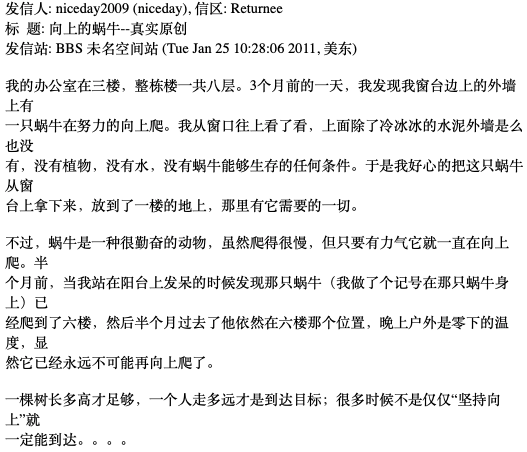
\includegraphics[width=.9\linewidth]{./pic/readme_20210520_095054.png}
\end{center}

当时状态下三大中文炒作出来的我表哥与我是可以结婚的状态,他们是希望我能够与我表哥结婚今生会比较幸福,还不是再去执着于硅谷职场——那个职场可能很肮脏。

这个态度以今天过来人的眼光回看,是非常公正的,但是它仍有一个前提就是:我亲爱的表哥必须是真心喜欢我的。我自已对我表哥的感情前面已经写得非常多了,我表哥这里是我今生永远最好的结局与归属,所以我这一方面的态度已经无需我再多说什么。

\begin{center}

\includegraphics[width=.9\linewidth]{./pic/readme_20210528_225603.png}
\end{center}

这个也与前面我说过的,参与三大中文枪手帖炒作一个人的人群里,有部分是真正的具体文艺才能的人,那么不可避免,这里面也是有心地纯正的人、又或者如当初的我般无法知晓与预测三大中文炒作cyber soup一个很普通女生的真正目的的人。 

\subsubsection{我的舅舅}
\label{sec:org2e46c07}

\begin{center}

\includegraphics[width=.9\linewidth]{./pic/readme_20210520_095645.png}
\end{center}

\begin{center}

\includegraphics[width=.9\linewidth]{./pic/readme_20210520_095719.png}
\end{center}

他们写过的舅舅的结局——晚景凄凉:两个侄女儿们并不感恩、到手的儿媳妇还将被他们三大中文逼良为娼、飞跑了(这事儿不是每个被逼的人都会就犯、他们三大中文也会有经历失败的时候比如临到逼我的份上他们就会失败)?!!!

因为我的心永远只属于我表哥一个人。我现在夏天是在还在加州这边打点儿工挣点儿学费和生活费用,等8月头秋季学期快要开学了(那时我现在的离婚程度也该彻底结束了吧?!!!终于可以恢复单身、可以真正好好与我表哥相处了,而不是总被我表哥打911),我是会回到我表哥所在的Pullman的土地上,回到我亲爱的表哥所在的WSU的校园里去读书的。虽然我今生最爱自己最后的这个《计算机》专业,但是我的生才表哥相比,我可能并没有天份走得更远、更何况这次回学校读书,我还想要去求、去争取一个将来远离硅谷三大中文的舆论场、加州硅谷它们三大中文逼良为娼根据地、回到我亲爱的表哥所在的学术圈清静地去度过余生,与我亲爱的表哥走到一起,真正活成自己想要成为的样子!

\subsubsection{我亲爱的表哥}
\label{sec:orge14ae3f}

\begin{center}

\includegraphics[width=.9\linewidth]{./pic/readme_20210528_231147.png}
\end{center}

这是10年12月回了学校一趟办OPT延期之后网上对舅舅、对我表哥等起来的涟漪。11年2月我同表哥说喜欢他想跟他后半生生活在一起的时候,表哥拒绝我的话是说他十年之内不会结婚。呵呵,十年过去了,亲爱的表哥,今年我们可以结婚了吗?

十年过去了,我们已经错过了十年;这次我会秋季回去读书,我不想再错过接下来的十年!我不想再错过我表哥、不想再错过与我亲爱的表哥生养孩子的机会,我不想接下来的十年还要过其它人的生活与人生。这像我的舅舅早就观察过评价过我的,我没有什么物质欲望,我只是力所能及地挣点儿生活费用满足基本的衣食住行就可以了。而特殊的人生经历,就决定了我必定想要求得精神上的满足,而这,只有我亲爱的表哥给予得了。 

从这一季站出来写的第一天开始,三大中文每天做的事情便是通过他们的媒体喉舌、故意炒作舆论,把舆论炒向他们所希望的方向。

但是自从2008年夏天舅舅亲自陪我驾车护送我来硅谷,从最开始的对于硅谷大城市生活、定居的无限向往,到15年来到加州之后的最近这几年,三大中文一次又一次地发动舆论想要逼良为娼,我看到了太多硅谷职场(专业职场与非专业职场)里被三大中文逼作了娼妇的种种罪恶与肮脏,现在我对加州硅谷大城市再也没有任何的向往,今生只要我亲爱的表哥还可以接纳我、只要我亲爱的表哥还能帮我把握我最后生育年龄的星点儿机会、能为我表哥生养一两个孩子,已然是我今生最大的幸福!

受够了现鬼窝的种种罪恶,哪怕只有最后两个月了,这个月底我也还是想要搬离这个恶磨一样的地方,哪怕在加州的这最后一个月住处比较难找,我仍然从未放弃希望,一定要7月底8月头回到我亲爱的表哥所在的Pullman的土地上,回到我亲爱的表哥所在的WSU的校园、回到学校去读书,永远远离这个极其肮脏罪恶的硅谷!!!

\subsubsection{我自己(两种结局)}
\label{sec:org47d879a}


舅舅又说,我家里人对我期望也挺高的,要我生活好,把自己的家人亲人照顾好!

我本能地觉得舅舅说要我生活好把自己的家人照顾好,当然是该先嫁给我亲爱的表哥,跟表哥结婚了,才是皆大欢喜的结局!!!

这些年里,我的舅舅对我说过的反话还少吗?这五大系列里,随便拎都可以拎出好多句出来!我的舅舅电话里当然对我说的是反话。 

\textbf{备注:}

我每次说我要把这些交待清楚,却也每次都也痛在自己心底,因为对我表哥的感情——因为就算现在、就算眼下退一万步说我表哥现在还不能够接纳我,也并不是说,我亲爱的表哥与我永远也不会走到一起,对于自己内心那场深入灵魂的遇见,我终究还是放不下、做不到淋漓尽致地决绝——我做不到不去顾及我表哥的感受而把所有我想说的关于三大中文错换人生逼良为娼的所有想法全部写出来。

如果我暂定8月头回我表哥学校的话,那还有两个月的时间、等我再好好想想、边写边想,看我最终能否把这个最痛苦也最头痛的问题自己梳理清楚(自己的个性是最好写的,而这个舅舅表姐参与其中的三大中文错换人生却也是我最陌生最头痛的、每次一想到要写这个甚至都把握不好自己的情绪)。

然后我也要打包准备搬家(至少这个月底先搬离现在这个鬼窝吧),8月头秋季学期快要开学的时候(7月31、8月1号)relocation到Pullman,这两个月再看看我还能写哪些、写到什么程度???

因为想要挣点儿生活费用,虽然挣得很辛苦,但并不是说这样我就会改变自己、随波逐流。我仍然会坚定地回我亲爱的表哥的身边,即便这次站出来写的这第五季可能写得断断续续,即便我现在可能不是很有时间来把它们写完写得很清楚,但是等我亲爱的表哥与我感情稳定、真正走到一起,有我亲爱的表哥的强大精神支撑,我是不会再惧怕任何的被当作什么样的人的,就算被当作某种典型,我想我也改变了一代人、向社会大众普及了一代人对于这个硅谷职场肮脏生存环境的认知。等有我表哥的强大的精神支撑,我想我将来还是有机会将这一切全部写清楚,哪怕是明年暑假(如果这个秋天能够与我表哥走到一起,并因为生养孩子而无法这次全部写完的话),我想等我真正获得更实在、更坚实的来自于我表哥对于我的精神支撑,我还是会最终把它们写完的,写到我觉得这个爱情故事、与对硅谷职场、三大中文舆论环境的社会认知前因后果全部交待清楚,可以真正称作写完的时候为止。 

今天会再写一点儿,争取把事情交待清楚——想要交待清楚,我是想要写出、表达出对我亲爱的表哥,不是12年4月舅舅口中说表姐们那样“自断退路”,我亲爱的表哥,永远是我最想要选择的路,包括当下、眼下、今年8月可望离婚程度彻底结束、我可以回到我亲爱的表哥所在的Pullman的土地上、回到我亲爱的表哥所在的WSU的校园里读书,或是回到我表哥曾经就读过的高中去当老师教书,陪我表哥一起走完余生。

所以,我这次站出来写的所有,仍然是以我随时准备好、随时都可以与我亲爱的表哥结婚为前提的。我的舅舅可能某些方面的事情做得不尽如人意,但这并不影响我亲爱的表哥与我的感情,作为亲人,我会包容舅舅所做过的所有的事情——我能很好地理解的、和我理解起来可能有点儿困难的,因为我亲爱的表哥,是我今生的归属,没有任何其它人可以替代。 

\section{2013 Summer Intern暑假实习(8)—— 还原当年三大中文舆论炒作的起始状态、立意与三大中文上它们自己作出的结论预测}
\label{sec:orgfe7fa98}

\begin{center}

\includegraphics[width=.9\linewidth]{./pic/backups_plans_20210514_121334.png}
\end{center}

你看,与小伙伴们的聊天,所有的小伙伴也都只是小伙伴而已呀,包括导师A与小伙伴D,除了是小伙伴之外,也并没有任何其它更多的情谊的。 

当我不自觉地把自己带入到了D的小伙伴的语境,不曾想,这里根本就没有自己的位置,D的小伙伴甚至直接说,实习生E“混血儿很聪明的!!!”

D的小伙伴说得我很错鄂和意外。 

\begin{center}

\includegraphics[width=.9\linewidth]{./pic/backups_plans_20210514_121704.png}
\end{center}

当D的小伙伴压根儿、从来都不把自己放在眼里,我申述了自己的立场,就算实习生E会被公司留下来,我也不觉得有什么,资本家的残食游戏而已。我能够把自己的事情做好便可以了。 

\begin{center}

\includegraphics[width=.9\linewidth]{./pic/backups_plans_20210514_122038.png}
\end{center}

就像导师A,实际上除了工作之外、除了这个暑假的实习之外,是与我没有任何关系、联系的。

\begin{center}

\includegraphics[width=.9\linewidth]{./pic/backups_plans_20210514_222850.png}
\end{center}

而我亲爱的表哥,如果今年我们能够走到一起,便是皆大欢喜、再好不过的事情(求仁得仁有何怨?而我也不会再计较、不会去索要先前舅舅曾经说过的关于说是我心里如果不平衡,可以向王夏华索要平衡的话)!

而如果我表哥或者是舅舅还再有任何的顾虑(比如十年了,如果它们三大中文逼良为娼还不能够得逞而要赶走王夏华职场的生存,如果舅舅也还是顺应三大中文的需求而把我继续朝三大中文逼我去当性奴的方向赶的话,我当然是不能服从、并要把所有的事实史实都摆出来的呀)而使得我亲爱的表哥仍然不能够与我走到一起,我们也该让社会舆论清楚地知晓这一美国近代历史上最为著名的逼良为娼恶意利用打压他人生存资源与炒作事件的呀。 

\begin{center}

\includegraphics[width=.9\linewidth]{./pic/backups_plans_20210514_124849.png}
\end{center}

我当时的想法、我当时对学校院里代课老师的理解,我也坦诚地分享给了自己的小伙伴们。

这些个几大系列的、分几次站出来写过的自己的传记,都自始自终地记载着自己的人格与人品,我从来都是坦诚,而不是你三大想要故意黑我的那样,什么谎话连篇,那些,更属于其它人吧。。

\begin{center}

\includegraphics[width=.9\linewidth]{./pic/backups_plans_20210514_115800.png}
\end{center}

我的项目还是写得很快的。周一过半,windows系统的就写得差不多可以用来测试了。

我问了先前长老B对面坐的senior,实验室里有没有我可以用来测试的机器。他说他不确定,但是可以帮助我确认一下。 

\begin{center}

\includegraphics[width=.9\linewidth]{./pic/backups_plans_20210514_115922.png}
\end{center}

在等待的时间里,我还是在继续进行着自己接下来的任务的。 

\begin{center}

\includegraphics[width=.9\linewidth]{./pic/backups_plans_20210514_120100.png}
\end{center}

后来的Linux系统的测试是如何进行的呢?

\begin{center}
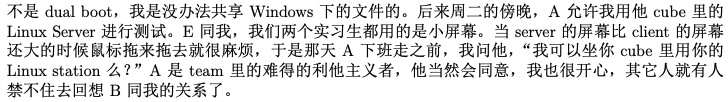
\includegraphics[width=.9\linewidth]{./pic/backups_plans_20210514_120348.png}
\end{center}

后来的Linux下的是在导师A的Linux station测试的。

\begin{center}
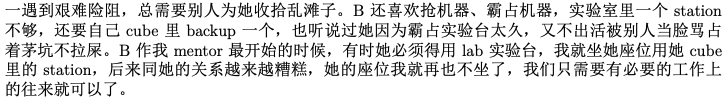
\includegraphics[width=.9\linewidth]{./pic/backups_plans_20210514_120603.png}
\end{center}

因为无法与前导师B建立起基础的合作关系,后来的我是一定不会再坐到长老B的位置上的。 

而后来与导师A的导师与被mentor、合作关系建立得比较顺利,所以我是可以坐到导师A的座位去进行测试的。

这也是从侧面反应了一个问题,就是与我亲爱的表哥的关系建立得很顺利,但是与两个表姐的关系却永远也建立不起来,这应该也是分人、与人的待人处世、以及专业素养等是相关的吧。 

以前的测试的历史没有写得很清楚。 

\begin{center}

\includegraphics[width=.9\linewidth]{./pic/backups_plans_20210514_121052.png}
\end{center}

MSTK log版块的测试的时候,测过了,导师A也还是比较开心的。 

\begin{center}
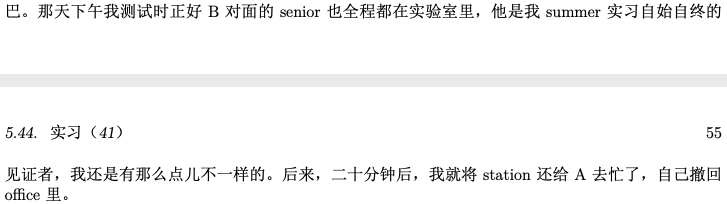
\includegraphics[width=.9\linewidth]{./pic/backups_plans_20210514_121200.png}
\end{center}

那个时候、那个项目的测试,我大概也就只测了十几分钟吧。

那个这个新的项目的周四的下午,导师A帮我reviwe的情况、进展如何呢?

\begin{center}

\includegraphics[width=.9\linewidth]{./pic/backups_plans_20210514_125439.png}
\end{center}

为什么导师A总想要找我的茬儿呢?

\begin{center}

\includegraphics[width=.9\linewidth]{./pic/backups_plans_20210514_125619.png}
\end{center}

那么这个,这只是一个小细节了,无关紧要。我帮导师A修改了一个小bug而已,谁也不会放在心上、没什么大不了的。 

\begin{center}
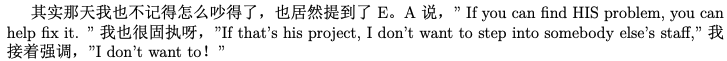
\includegraphics[width=.9\linewidth]{./pic/backups_plans_20210514_125725.png}
\end{center}

导师A居然会指使我去找实习生E项目里存在的bug?我没有这份意愿。 

就要到实习的最后一个周了,感觉还没有机会能够多学到东西,就不得不要回到学校里去了,那么我就想问一下组长C,我的实习可不可以再延长一个周,争取能再多做一个小项目。 

\begin{center}

\includegraphics[width=.9\linewidth]{./pic/backups_plans_20210514_115101.png}
\end{center}

\begin{center}

\includegraphics[width=.9\linewidth]{./pic/backups_plans_20210514_115223.png}
\end{center}

\begin{center}

\includegraphics[width=.9\linewidth]{./pic/backups_plans_20210514_115233.png}
\end{center}

这些话是前还在公司里吃晚饭、尖人还允许自己在公司里吃晚饭的时候,一天傍晚吃晚饭的时间我在表姐的坐位里问表姐的。 

\begin{center}
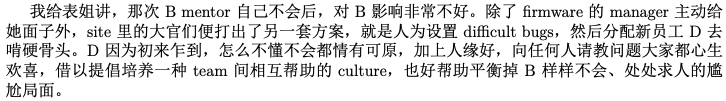
\includegraphics[width=.9\linewidth]{./pic/backups_plans_20210514_115523.png}
\end{center}

用正式员工D来给我先前的导师mentor senior长老B洗地。 

亲爱的读者,写到这里,我已经无心再继续写下去了。

不是写到这里,我无心再写下去了,而是(像我这样沉浸式思维会翻来复去地去想,有时候就会难免)觉得如果我亲爱的表哥不够喜欢我、无法喜欢和接纳我,我可以就没有信心和勇气再写下去了吧。 

原本,比如我亲爱的表哥接起电话,我表哥对我多说几句话,我都会开心很久,都有很大的信心接着写下去、写完;但当我越来越找不到支撑、而我与我亲爱的表哥的联接与信任、被三大中文媒体一再反方向作用力平衡、被大表姐一再从中作梗的时候,我就还是会受到这些环境的影响而显得很难再坚持写下去了。 

但我还是会尽自己的最大努力把自己的思维逻辑和立场阐述清楚。所以,接下来的部分,如果我还在接着往下写、接着更新的话,就让我们来试图回归当年的、我所理解和了解到的所有的真相。

首先,我自己的个人立场最重要。我仍然会回pullman,但在我亲爱的表哥主动联系我(这个或许会很快发生,如果我亲爱的表哥这些年是真心真意喜欢我的话,恩我相信这一点儿,我表哥如果有他喜欢的人,这些年里一定是我!!!或许永远不会再发生,如果他确实从来就不曾真正喜欢过的话,但是这点儿我不相信、现在不相信:我不相信我表哥从来不曾喜欢过我,这话只是大表姐给我洗脑的话)之前,我不会再主动与这家人有任何联系了(为我自己的安全考虑——我不希望再收获来自于舅舅或者是表哥的任何911或者更甚一步的行动了)。我想回Pullman读书,是我自己厌倦了硅谷大城市的肮脏、喧嚣,与亲近宁静小城市和大自然的需求、和我自己心底一份坚守自己爱情的信念与执着,以及想要以后永远远离硅谷、争取能够在小城市、学术圈勉强生存的愿望与努力。

是有这个愿望,但六月份回去了大家都在放暑假(学校院系里的老师、工作人员们),我申请学校联系老师都不太方便,我觉得我可能还是在这个硅谷再多呆两个月,到八月头回去,立即联系老师,能够秋季上学最好,实习不能秋季上学可能会往后拖一个学期吧。不过我会尽最大努力(如果实在申请不到任何奖学金、或是实在录取不了)秋天回学校读书(秋天脑袋比较清醒一点儿)。这两个月(六月七月,因为这个月底我一定会搬家)我会尽量再挣些学费生活费用供接下来上学用。因为还有两个月才回我表哥所在的Pullman的话,那这两个月我还是会因为我亲爱的表哥、因为与我表哥之间的爱情信念信仰、以及我表哥学校的运动队运动精神支撑而接着往下写,写到有一天我实在、再也找不到任何动力、或是再也找不到任何爱情信仰或环境的支撑为止。但可能不是每天都能更新很多,就每天、或是两三天,能写一点儿出来就更新一点儿吧。

三大的黑:他们黑我的时候,一如当年他们会故意禁网,故意制造人民群众不敢发声的网络场景,他们会禁我的IP,并发动每次为期一天左右的可以合理猜测的对我集中火力的黑,比如拿我个性中的某些缺点来故意黑我、集中火力地故意黑我;不留余地地!

我先前的观点,还曾想过要不要从王夏华处要结婚彩礼呢?现在,那些彩礼什么的我都不再想了。求仁得仁,能够得到我表哥我就很知足了。只求我不负任何人,就可以了,用我的舅舅12年4月他当作新闻发布会上的观念信条来要求自己。

12年、08年夏天舅舅把我送到加州硅谷人间繁华地来体验大城市的繁华。十多年里,我终于是看透了大城市繁华背后的虚幻、对大城市终于是不再向往、没有留念、甚至想要远走离去、去避开它的喧嚣纷杂。

我想要离去,那我想要去哪里呢?当然是想去表哥的城市去生活呀!

当我厌倦了城市的喧嚣纷杂与浮躁,我想念菁菁校园的静谧沉静,我想要回到表哥的故乡、舅舅也喜欢的、表哥工作的校园坐落的大自然中去!

作为一个农村长大的孩子,我喜欢广袤的大自然,我喜欢雨过天晴的滋润清新,我喜欢雨后、夜幕降临下的青草味道;

小时候二姐带我们去叔叔家做客,我们一定会选择下雨天去,应该下雨天去叔叔用他的渔网打鱼会比较有渔获,而我就是那个喜欢跟着叔叔去广袤的大自然中去呼吸新鲜空气的、捡渔虾的小P孩;

小时候同爸爸出去打鱼的时候夜晚里夜幕降临露水落下、滋润清新的夜幕下的青草味道,这些青草味道、雨过天晴的滋润清新都已经深深地刻在了我的灵魂深处;

我喜欢大学时期武汉的梅雨季节的雨水,这些雨水滋养着我的灵魂(和12月7日的校园广场绘画展,艺术陶冶情操,我的心灵得到洗涤与滋养)

2005年夏秋、当实验室一定不再是我的选择,我选择了去山青水秀的广西养病,帮助自己早日从困难中摆脱出来;

2013年夏天我终于鼓足勇气去锻炼身体(去山林中hiking),我把自己锻炼得比较好,我也把自己工作时的精神状态调整得比较好。

大家也看见了,我对自己这个认得的舅舅的看法是一分为二的。

今年的3月13、14日那个周末,我开始读了自己当年、早年传记中的大部分内容,可以清楚地读出当年那个幼稚的自己。所以,就像我自己所能够感觉到的舅舅曾经给予过的暗示,今年的3月15日早上八点零几分,我终于是鼓足勇气、于11年11月给舅舅打过一个电话(那年我的爸爸出意外,电话里我问舅舅我可不可以与表哥结婚、哪怕先只把结婚证领了都行,舅舅说表哥的感情不到位)多年以后再打电话给我的舅舅,我播通了舅舅的电话。 

电话里我向舅舅对自己当年的幼稚行为道歉(比如11年5月底回去也回去了,不听舅舅到底怎么说,一回家看见地上的东西转头就走等幼稚行为,电话里我并没能对舅舅讲这些我所认知的道歉细节)。舅舅倒也没有计较。电话里我两次问及舅舅“我表哥呢?!!!”这些年里,唯有那个心心恋恋的表哥仍然是她心底最深的眷恋、是她战胜所有硅谷三大中文逼良为娼黑势力的源动力,舅舅只答说他不知道。那我也只能主动事后自己联系过我表哥。问及我想像当年的表哥一样读个博士学位,舅舅却要坚定地把我锁定在硅谷,答说我想读博士,我可以在加州硅谷读博士——这会让我一再去想,舅舅电话里说要我留在硅谷的目的是什么?08年舅舅开车护送陪我前往硅谷的路上,他不是对我一再重申他觉得小城市的生活比较安静静谧吗?更何况,回到小城市,回到我表哥所在的城市,老大不小的我亲爱的表哥和我两个人也才能真正走到一起、重新组建家庭life也才能够move on的呀?!

一方面舅舅说,他不知道我表哥到底在哪里;另一方面,舅舅又不免提及表哥,舅舅电话里在我面前表扬我表哥说我表哥“你表哥他很聪明、也很有报负!”我亲爱的表哥、这些年里,在我这里自然是极其聪明、又待我很好的强大存在、作为源动力、精神动力支撑了我这过去的这些年!那舅舅口中,我表哥的报负是什么呢?

这些年里,因爱我表哥生恨也罢,我恨过舅舅、狠狠地恨过舅舅(现在已经没有那么恨了)、对大表姐王夏华做过的很多事情不平衡过,但一如三大中文所了解到了,我亲爱的表哥在我这里,从来都是一个完美无缺的存在;他们都知道,我对别人对别的任何人有任何的看法,我从来不曾说过我表哥有任何的不好,因为我亲爱的表哥,待我从来都是极好的——那场深入骨髓、灵魂深处的遇见,又怎么可能是俗世里曾经将就的婚姻对象、比如会随便发泄他的怒气脾气会随便对他自己的女人下狠动手打人的前夫可以随便相提并论的?!!!

就像我先前所写到的,我这辈子,什么时候都是随时准备好、随时都可以与表哥结婚的状态!!!

所以,我一定要回到我表哥的身边,哪怕只是呆在我表哥所在的Pullman WSU校园里去读书、去读一个不是很热门,但仍然极有意义的专业!

\begin{center}

\includegraphics[width=.9\linewidth]{./pic/readme_20210516_102713.png}
\end{center}

如果我的表哥十年了还不结婚,那我以后也可以不再结婚,直到表哥先找到他的幸福为止!因为我表哥曾经待自己的好,我愿意用自己的余生作陪葬,一如我表哥先前曾守候过我的幸福,我愿意守候亲爱的表哥余生的幸福!!!

\begin{center}

\includegraphics[width=.9\linewidth]{./pic/readme_20210515_095559.png}
\end{center}

这里,我想,我更想表达的是,对于我来说那场深入骨髓的遇见,我亲爱的表哥这里我相信也是爱情的;但退一万步,如果我表哥是把它当友情处理的,我同样尊重表哥待我的好,一如那场遇见成为开在灵魂深处的花,静静绽放在无数个午夜梦回的夜里、绽放在寂莫生活的思恋里。哪怕是一场美好的回忆,也都将永远被珍藏!!!

我的舅舅自然是有着不同处理的,他十岁随二外公离家避开斗地主的斗争而逃走闯社会,他的社会阅历与认知、他的透彻都迫使他站出来、帮助有可能不善处理感情问题的表哥、有可能因为过于善良不忍心拒绝我的表哥摆脱来自于三大中文社会舆论压力与困扰——这个在2010年12月、2011年1月2月是客观存在的:因为当时三大的舆论炒作已经分为了两个方向:如果我表哥是真爱我,待我那般好,我与我表哥遇见的那场告别、我表哥牵着我的手把我送出来等等,都成为人们内心深处所向往的美好爱情的投注、投注关注在我表哥与我身上,很大一部分人也都认为我表哥与我当时应该会很快就能结婚的(而我自己当时对于我表哥的认知还有些傻傻分不清楚而已);另一方的舆论,却是认为这个家族出过“王妃”,熟知三大中文逼良为娼黑色产业链的人、三大内部人士也会一再去追问和印证:我表哥与我到底是爱情、还是只是拿爱情当幌子借用他们三大中文黑势力帮助2006年与我来美读博士同期进入美国的我舅舅的亲侄女王夏华谋取职场生存?

我表哥与我之间的亲密是有目共睹的,不需要任何再多的语言。所以我也从来没有认为与表哥的那场告诉:我亲爱的表哥与我,任何一方有任何的过错,这都是人类灵魂深处最为纯真的情感!!!不是我的舅舅随便一句一顶“不择手段”的帽子就能把人打倒的!!!

只是我的舅舅,接下来帮助表哥摆脱舆论压力的处理办法,便是在继2011年5月底傍晚我表哥带我回到家后一看见被舅舅摆在满地的东西便扭头就走了(还把当年幼稚的自己气得要死要活,恨不得一脚加足油门把车开下山崖下,让我表哥和舅舅报撼终生)之后,继2011年7月我受当时“朋友圈”的蛊惑而写邮件给我表哥表达想要与表哥结婚之意后,我的舅舅邮件暴力警告我他要打911!

而我也便直冲冲地撞上去了回去找舅舅报仇雪恨了——因为舅舅的警告过于严厉,我接受不了:与其恨痛在心底、不如淋漓尽致地回家找舅舅决一了断!于是有了11年8月头我有工作后冲回去一言不发等舅舅打911——而同时,我亲爱的表哥一再用行动表明他的立场:他仍然是喜欢我、是希望我能够做他房间女主人的!!!

我的舅舅播打911的意义,我的总体立场是,舅舅借助这样的911法律暴力,便是把所有任何人、任何一方可能有的过错、与当时的社会舆论压力全部强加到了我一个人的头上,这是社会阅历丰富的舅舅对我表哥最本能的保护,但这也是当年我亲爱的表哥眼中的少女心小弱弱无论如何也都还承受不了承受不起的!

这里,我们再来分几个方面的意思来分析和讨论舅舅播打911的几个方面的意思。 

舅舅又说,我家里人对我期望也挺高的,要我生活好,把自己的家人亲人照顾好!

我本能地觉得舅舅说要我生活好把自己的家人照顾好,当然是该先嫁给我亲爱的表哥,跟表哥结婚了,才是皆大欢喜的结局!!!

这些年里,我的舅舅对我说过的反话还少吗?这五大系列里,随便拎都可以拎出好多句出来!我的舅舅电话里当然对我说的是反话。 

\textbf{备注:}

今天会再写一点儿,争取把事情交待清楚——想要交待清楚,似乎也好难交待得清楚、这里面有亲情、有爱情、有亲人间的不能理解、也有不亲的人对自己的利用。

我每次说我要把这些交待清楚,却也每次都也痛在自己心底,因为对我表哥的感情——因为就算现在、就算眼下退一万步说我表哥现在还不能够接纳我,也并不是说,我亲爱的表哥与我永远也不会走到一起,对于自己内心那场深入灵魂的遇见,我终究还是放不下、做不到淋漓尽致地决绝——我做不到不去顾及我表哥的感受而把所有我想说的关于三大中文错换人生逼良为娼的所有想法全部写出来。

如果我暂定8月头回我表哥学校的话,那还有两个月的时间、等我再好好想想、边写边想,看我最终能否把这个最痛苦也最头痛的问题自己梳理清楚(自己的个性是最好写的,而这个舅舅表姐参与其中的三大中文错换人生却也是我最陌生最头痛的、每次一想到要写这个甚至都把握不好自己的情绪)。

然后我也要打包准备搬家(至少这个月底先搬离现在这个鬼窝吧),8月头秋季学期快要开学的时候(7月31、8月1号)relocation到Pullman,这两个月再看看我还能写哪些、写到什么程度???

\section{成长的故事 -- 我和表哥}
\label{sec:org804f892}
\begin{itemize}
\item 2011年11月4日,当三大中文媒体对我的人肉已经伤及我自身生活,我必须站出来澄清自己, in Part 1, (San Jose, CA);

\begin{center}

\includegraphics[width=.9\linewidth]{./pic/dreamer1.png}
\end{center}
\item 4/19/2012 - 6/17/2012, in Part 1, 第二次写至统计专业OPT实习结束(San Jose, CA);

\begin{center}

\includegraphics[width=.9\linewidth]{./pic/dreamer2.png}
\end{center}
\item 2014年夏天,写于SJSU Library (San Jose State University Public Library, San Jose, CA)

\begin{center}

\includegraphics[width=.9\linewidth]{./pic/dreamer30.png}
\end{center}
\item 2/13/2015 - 12/17/2015(?, Moscow, ID; either and or not San Jose State University Public Library, San Jose, CA)

\begin{center}

\includegraphics[width=.9\linewidth]{./pic/dreamer3.png}
\end{center}

\item I will reorganize the four pdfs, and emphasize keys issues and situations of the whole process, while at the same time to help major population understand what's going on, and what's inside opinions. 虽然这个成长的故事系列是以2011年当三大中文网站(mitbbs.com, wenxuecity.com and backchina.com)中文媒体对我的人肉与网上评论伤及我的正常生活时,我站出来开始写自己的自传,并分四次在四个不同的时间段,不同舆论或事件压力下或是网上澄清,或是网上求助以便能帮我泄掉一部分当时自己的压力,分四次于不同的地点纪录了的自己的主要生活,纪录到2015年计算机硕士学位结束。
\item 这一次,这里,我会以事件主要人物及其相关主要事迹的人物列传、或/和大事记、大冲突记的形式来重新组织语言,重述我的整个成长史与大事记、大冲突记,来帮助自己成长、并帮助社会大众认清事情所有环节真相的目的。但鉴于时间有限,我会以剧情梗概的形式每天大致纪录与一个相关人物某件或某几件事的进展、或一天一两个主要事件,并将已经完成了的四个部分作为原始事件纪录的细节参考供索引,并争取做到每日更新一篇,到我把先前与这个教授舅舅的所有冲突的这件事情具体讲述清楚,以供大家共同去探讨事情的真相到底如何,有一个更能为大家所接受或理解的底层社会小人物的心灵成长史。
\end{itemize}

\section{2013 Summer Intern暑假实习(6)—— 交叉项目:人际交叉、公司栽脏爆点、炒作职场非正常男女关系舆论}
\label{sec:org70ac7ef}

前面写到了:实习生暑假实习期间正常更换实习导师、被三星公司高层组长C等刻意安排、制造舆论、炒作成了:实习生我处理不好与三星公司正式员工、mentor senior长老B的职场人际关系,迫使公司不得不为我这个事端制造者更换了导师。 

\begin{center}

\includegraphics[width=.9\linewidth]{./pic/backups_plans_20210511_101118.png}
\end{center}

上个周是属于实习生实习期间换mentor、公司自导自演又上演了一出三在中文炒作舆论的燃点爆点。

\begin{center}

\includegraphics[width=.9\linewidth]{./pic/backups_plans_20210511_102103.png}
\end{center}

公司里的领导自己的样子倒是做得很好的,该道歉的道歉,但是被他们故意炒作、作贱、被剥夺了生存资源的职场年轻女性的生存空间呢?是他们为官的假惺惺一句道歉就可以解决得了的吗?

\begin{center}

\includegraphics[width=.9\linewidth]{./pic/backups_plans_20210511_102539.png}
\end{center}

更何况,就像表姐所陈述清楚的,她只是善常体察上意,将上层领导们需要、想要她帮招进来的那些个公司里的易燃易爆品招募了进来。

\begin{center}

\includegraphics[width=.9\linewidth]{./pic/backups_plans_20210511_102727.png}
\end{center}

而他们、公司上层自然是清楚地、仔细地打听过他们所招员工(比如那个暑假专门用来拖住我、对付我的、缺乏专业素养的长老B)的人品、素质、工作表现等方方面面!!

你以为他们这次的换导师事件只是各种情形之下的一件事发突然吗?

不,他们有专业的故意制造燃点爆点舆论踢爆炒作小分队、他们接下来仍然会(利用他们为我组装的小伙伴队伍的口舌、警犬尖人、表姐等)一再造谣、一再人为刻意制造燃点、爆点,并利用合用三大中文媒体喉舌的力量将这股舆论彻底炒爆、炒出他们三星公司所想要达到的他们曾经多么地仁义、公道、曾经多么仁慈地站出来救助过的人道主义立场!!!

接下来,我们还是先看项目上的进展。 

\begin{center}

\includegraphics[width=.9\linewidth]{./pic/backups_plans_20210511_105354.png}
\end{center}

这里应该是存在一些笔误:就是这是前导师长老B一个周前给布置的交叉项目,现在是暑假后半段新换导师、前文称呼正式员工A帮忙review. 

\begin{center}

\includegraphics[width=.9\linewidth]{./pic/backups_plans_20210511_105634.png}
\end{center}

\begin{center}

\includegraphics[width=.9\linewidth]{./pic/backups_plans_20210511_105715.png}
\end{center}

这里的笔误是,这个项目不是要从一个文件,而是从多个文件。回忆起来某些不太显眼不太重要的事件的先后顺序可能会有错乱,在所难免。这个小细节就此指出,不必过于在意。 

那么这个上个周所布置的交叉项目、前导师长老B所留下的上个周的项目,新导师A会如何帮我review呢?

\begin{center}

\includegraphics[width=.9\linewidth]{./pic/backups_plans_20210511_110111.png}
\end{center}

换导师后新一周的周一还是周二的中午偏下午一两点钟(?),新导师A就帮稍微点评了一下代码乱在哪里,可以先从哪些方面作些改进。

\begin{center}

\includegraphics[width=.9\linewidth]{./pic/backups_plans_20210511_110130.png}
\end{center}

\begin{center}

\includegraphics[width=.9\linewidth]{./pic/backups_plans_20210511_110510.png}
\end{center}

\begin{center}

\includegraphics[width=.9\linewidth]{./pic/backups_plans_20210511_110559.png}
\end{center}

从小喜欢学《数学》、《化学》等非语言文字学科、学过《统计》硕士专业,经历过统计专业29个月的OPT实习,我应该总是对自己分析解决问题的能力还是比较肯定、有着很大程度上的自信的吧。 

\begin{center}

\includegraphics[width=.9\linewidth]{./pic/backups_plans_20210511_110329.png}
\end{center}

这里,我又一次自信地(或者说是自大地)估计了一个一个小时之内解决掉导师A所提出的建议问题的(改混乱代码成为一个module),却意识不到这是一个考验的开始。 

\begin{center}

\includegraphics[width=.9\linewidth]{./pic/backups_plans_20210511_111340.png}
\end{center}

但那时,我真的认为我不是在骄傲,而是心里面有一种急——如果这个导师的编程能力真的很强大,那么作为我亲爱的表哥眼中少女心小弱弱的我,是很想要抓住这个机会多从这样一个职场专业人士的guidence里多学习点儿新知识、新经验或者是能够被他培养出多一些计算机专业里的能力的。

我很急,我想要尽快、估莫着一个小时左右把事情做完,好可以把这个项目干完了结、好可以从导师A那里请他帮忙想出、我可以索要得到新任务、或者更多的任务与专业锻炼。 

\begin{center}

\includegraphics[width=.9\linewidth]{./pic/backups_plans_20210511_111704.png}
\end{center}

但是很显然,作为python语言的小儿科弱弱,我还是严重低估了它的难度,修改的过程中也出现过各种各样的问题,一两个小时后到那天下午三四点钟的时候,我已经有些沉不住气,跑去同新导师A交换一下意见了。 

\begin{center}

\includegraphics[width=.9\linewidth]{./pic/backups_plans_20210511_111728.png}
\end{center}

我这样跑去问导师A,是有点儿打扰他了。但当时的自己已经感到压力了,需要与导师交换一下观点意见、作些调整吧。

\begin{center}

\includegraphics[width=.9\linewidth]{./pic/backups_plans_20210511_112426.png}
\end{center}

新导师A说等他忙完再去帮我看看。而我、稍微减压后还是得回去继续修改自己的代码。 

\begin{center}

\includegraphics[width=.9\linewidth]{./pic/backups_plans_20210511_112554.png}
\end{center}

又过了约两个小时左右,当傍晚六点钟,导师A不得不下班的时候,他过来察看我的进展。 

\begin{center}
\includegraphics[width=.9\linewidth]{./pic/backups_plans_20210511_112718.png}
\end{center}

恩,又过了两个小时,又整了两个小时之后,我终于是把那个python module的入门级知识点、考点儿给过了!

\begin{center}
\includegraphics[width=.9\linewidth]{./pic/backups_plans_20210511_110559.png}
\end{center}

新导师A还比较开心,他那天已经到下班时间要回家了,他答应第二天就帮我review. 新导师A会帮我想出来、会安排我做的下一个项目会是什么呢?到那时,我应该还是很开心很向往的吧,一如当年几个月前的春天AI人工智能课结束、清楚地感受了一个学期这门课代课老师的分析能力与授课知识点的透彻性,我已经向代课老师上课提问示好(明示问题示好),表达了我跟他做科研的兴趣,期望以后能有机会跟他一起作课题!

\begin{center}
\includegraphics[width=.9\linewidth]{./pic/backups_plans_20210511_114253.png}
\end{center}

那个周二的下午,三四个小时,只为解决、fix掉一个learning curve偏低的python的一个基础级的module入门考点bug。那三四个小时,自已的亲身体会、真切感受如何?

\begin{center}
\includegraphics[width=.9\linewidth]{./pic/backups_plans_20210511_114322.png}
\end{center}

这里,当新导师A给我更多的时间让我学着去自己解决问题,我能够感受到自己需要努力,也能够做到在心里鼓励自己更加努力。 

\begin{center}
\includegraphics[width=.9\linewidth]{./pic/backups_plans_20210511_114411.png}
\end{center}

这里确实是一个基础,如果导师A同任何其它庸俗碌碌辈一样、同先前长老B凡事不会就去问其它组其它同事一样,那我们实习生实习期间的专业能力、是很难得到成长与提升的。 

这个基础——互相站在对方的立场上试图去为对方想一想、并相信对方的做法一定是为自己好的、是有他自己一定道理的,确实是垫定了实习期间这个导师与实习生我之间相互理解信任的mentor-guidence合作基础。

我们来回忆一下我亲爱的表哥与我建立信任基础、爱情基础、到树立起坚定的爱情信念的那些个感动瞬间。 

\begin{center}
\includegraphics[width=.9\linewidth]{./pic/backups_plans_20210511_115910.png}
\end{center}

2010年2月,当《统计》专业的我硕士毕业,就要前去加州找工作了,走之前路过表哥家,把一两样不太重要的东西留下,却发现我亲爱的表哥从他的车里钻出来,送我出门呢!

\begin{center}
\includegraphics[width=.9\linewidth]{./pic/backups_plans_20210511_120022.png}
\end{center}

但是到了加州之后,我对我亲爱的表哥爱情的点点星火就被大表姐给亲手掐灭了。 

\begin{center}
\includegraphics[width=.9\linewidth]{./pic/backups_plans_20210511_120208.png}
\end{center}

\begin{center}
\includegraphics[width=.9\linewidth]{./pic/backups_plans_20210511_120306.png}
\end{center}

\begin{center}
\includegraphics[width=.9\linewidth]{./pic/backups_plans_20210511_120425.png}
\end{center}

\begin{center}
\includegraphics[width=.9\linewidth]{./pic/backups_plans_20210511_120500.png}
\end{center}

\begin{center}
\includegraphics[width=.9\linewidth]{./pic/backups_plans_20210511_120655.png}
\end{center}

\begin{center}
\includegraphics[width=.9\linewidth]{./pic/backups_plans_20210511_120730.png}
\end{center}

\begin{center}
\includegraphics[width=.9\linewidth]{./pic/backups_plans_20210511_120816.png}
\end{center}

\begin{center}
\includegraphics[width=.9\linewidth]{./pic/backups_plans_20210511_120902.png}
\end{center}

\begin{center}
\includegraphics[width=.9\linewidth]{./pic/backups_plans_20210511_120952.png}
\end{center}

\begin{center}
\includegraphics[width=.9\linewidth]{./pic/backups_plans_20210511_121705.png}
\end{center}

\begin{center}
\includegraphics[width=.9\linewidth]{./pic/backups_plans_20210511_121521.png}
\end{center}

等我10年12月再回去与我表哥相处两天,我的大表姐已经永远也无法再掐灭我心中的爱情信仰了!!!

你看,与新导师A三星公司实习期间的这个mentor-guidence合作基础、友情基础,与我亲爱的表哥与我相处之初的爱情基础相比、与先前导师mentor senior长老B的不能理解、尊重与信任相比、与大表姐们无法建立起很好的联接相比,这份基础从第一个小事件就真正建立起来了。 

这里,我将与不同人之间建立信任的基础列在一起,但这并不是说,我就又傻傻分不清楚,新导师A与我亲爱的表哥之间的本质区别。因为那个时候,生活的经验、从我的舅舅那里曾经的教诲已经教会了我什么样的人是不能搅在一起的!

\begin{center}
\includegraphics[width=.9\linewidth]{./pic/backups_plans_20210511_122404.png}
\end{center}

2003年10月进到实验室人口密集集中的地方,我有点儿往人海里掉的时候,我没有掉进我们明确已婚的师兄那边!

\begin{center}
\includegraphics[width=.9\linewidth]{./pic/backups_plans_20210511_122514.png}
\end{center}

2007年左右,当已婚属马师兄与他老婆谢姐姐之间出现感情问题,当一个秋冬的晚会上谢姐姐要求当年的男闺密送她回家后,我曾特意提醒男闺密,不可以掉进别人感情的旋涡里!

\begin{center}
\includegraphics[width=.9\linewidth]{./pic/backups_plans_20210511_122431.png}
\end{center}

2008年春天,当有我机会见到我的舅舅,曾不经意侧面征求舅舅意见的我,便被经历过世事、犀利透彻的舅舅一语点醒并警钟长鸣!!!

\begin{center}
\includegraphics[width=.9\linewidth]{./pic/backups_plans_20210511_123400.png}
\end{center}

那么,亲爱的读者,你以为,这次,在三星公司这个site里实习的这个暑假,在三星公司collect的易燃易爆品(已婚导师A,与未婚小伙伴D)面前,我又一次地被引爆了吗?

我没有!

在我亲爱的表哥与我的感情世界里,我从来不曾被新导师A引爆(他在我这里没有任何立足之地,除了作为实习生的导师,作为三星公司招聘进去的正式员工,当领导上层安排了他mentor我,他应尽的职责、与基本义务)。因为我心有所属,我有爱情信仰,我永远不可能背叛我亲爱的表哥的呀!

真正引爆舆论的是,真正有过的只是,曾经引爆舆论的、曾经三大中文媒体故意炒作过的,三星公司的舆论民间网红广告创意、三星公司内部舆论炒作、操控手们的布点、布阵(栽脏的小伙伴队伍,与三星公司site里的各种托儿各个托儿们)与栽脏!!!这此,细节会一一再述,就当就此提及而已。

那么解决这个小bug的第二天(周三),新导师A对我的交叉项目的review,就像那个交叉了前后两个暑假实习期间导师的人际关系一样,交叉平衡了组里的人际关系,并在我的人生经历里,又一次地挑战了自己个性中的脆弱面,成为一件我期待着新项目的周二傍晚又一个意料之外的review与人际感受!

\begin{center}
\includegraphics[width=.9\linewidth]{./pic/backups_plans_20210511_124702.png}
\end{center}

这是一段的客观描述当时工作组、工作的三星公司那个site里的情况,也难免会有一丝一毫的个人感受,因为对于接下来(新——到这里大家都知道换导师了,以后便就是导师A了)导师A对于我的批评——我接受起来是有困难的!

\begin{center}
\includegraphics[width=.9\linewidth]{./pic/backups_plans_20210511_125033.png}
\end{center}

导师A帮我review项目很慢。上个周一个周的时间早就写完了那个交叉项目,但是A是一拖再拖,这不,调节平衡组里的人际关系也罢,一拖就拖到了周三了——新的一个周已然又已经过半了!!!

导师A对我的批评是什么呢?他嫌我急?!!!可是我不急,我能有机会多做几个项目吗?!

\begin{center}
\includegraphics[width=.9\linewidth]{./pic/backups_plans_20210511_125118.png}
\end{center}

导师A对我的这点儿批评——如果称之为批评的话,说得是客观公正,表达的或许也是他曾经作为计算机专业入门者时、或是进阶过程中的亲身感受与体会,但在我亲爱的表哥眼中的少女心小弱弱眼里,这就是赤裸裸的批评了呀,接受起来还是好困难的!

弱弱眼中导师A的review是什么情况、状况呢?

\begin{center}
\includegraphics[width=.9\linewidth]{./pic/backups_plans_20210511_125437.png}
\end{center}

我觉得他总是想找理由批评我。

\begin{center}
\includegraphics[width=.9\linewidth]{./pic/backups_plans_20210511_130349.png}
\end{center}

这里我们仍然可以一分为二地看待。就是一方面导师A作为这个组里的员工,确实有照顾我前导师mentor senior长老B的主观个人感受,而在那个旧新导师更替的关口,一定要批评我一下,这在先前当长老B与我的subversion的提交傻傻分不清楚的时候他也曾站出来平衡过。另一方面,我们仍然可以看作我的项目确实存在着怎样的问题。 

我们先来回顾一下,我亲爱的表哥眼中的少女心小弱弱成长的历史上、那几次经受振聋发溃的批评的历史案件!

\begin{center}
\includegraphics[width=.9\linewidth]{./pic/backups_plans_20210511_161158.png}
\end{center}

国内硕士研究生时导师在我开题告上对我的严厉批评,让我倍受痛楚,只想要做个冷血的学生,只求能够正常硕士毕业就好!

\begin{center}
\includegraphics[width=.9\linewidth]{./pic/backups_plans_20210512_100225.png}
\end{center}

\begin{center}
\includegraphics[width=.9\linewidth]{./pic/backups_plans_20210512_100246.png}
\end{center}

\begin{center}
\includegraphics[width=.9\linewidth]{./pic/backups_plans_20210512_100345.png}
\end{center}

\begin{center}
\includegraphics[width=.9\linewidth]{./pic/backups_plans_20210512_100319.png}
\end{center}

\begin{center}
\includegraphics[width=.9\linewidth]{./pic/backups_plans_20210512_100159.png}
\end{center}

11年2月当我回到家里向我亲爱的表哥表白,当我的舅舅故意将一顶顶罪恶的帽子向我头上砸来,当我的舅舅批评我的时候,我是全然不能接受哪怕是来自于自己深深信任的舅舅的严厉批评的!!!

\begin{center}
\includegraphics[width=.9\linewidth]{./pic/backups_plans_20210512_100728.png}
\end{center}

当那时我的舅舅对我的批评真正转化成自己可以意识到、可以落实到行动上的改变时,是又经历了一番自己的经历与领悟之后的事。 

\begin{center}
\includegraphics[width=.9\linewidth]{./pic/backups_plans_20210512_101244.png}
\end{center}

\begin{center}
\includegraphics[width=.9\linewidth]{./pic/backups_plans_20210512_101141.png}
\end{center}

12年5月,当我深爱的、我亲爱的表哥与播打了911之后,我恨过我表哥吗?当时的小弱弱是如何处理、过渡这段被自己亲爱的表哥播打911的事情呢?

\begin{center}
\includegraphics[width=.9\linewidth]{./pic/backups_plans_20210512_101333.png}
\end{center}

那时,被关在被自已称为“人间炼狱”的地方,只要我能够找出自己个性上存在的缺点,我就可以继续一如既往地相信我的亲爱的表哥!这就是我亲爱的表哥在我这里强大而又无卸可击、又给予着我深深爱恋的我亲爱的表哥在我这个当初的我亲爱表哥眼中的少女心小弱弱的强大存在!

\begin{center}
\includegraphics[width=.9\linewidth]{./pic/backups_plans_20210512_102518.png}
\end{center}

\begin{center}
\includegraphics[width=.9\linewidth]{./pic/backups_plans_20210512_102616.png}
\end{center}

而到后来,当我再长大一点儿、成熟一点、全然明白,我亲爱的表哥从来都是为我好、从来都是把选择权留给我、让我自己来作选择,便最终理解了我的舅舅和我亲爱的表哥最初的冷血、看似残忍做法。

我亲爱的表哥所曾给予我的这份爱,是这个世界上再也没有其它任何人可以给予我的,是我内心的深深索求与需要,所有今天的我选择回到我亲爱的表哥的身边,是再也没有任何其它外力可以阻止得了的。这是现在的最真实的感受。 

\begin{center}
\includegraphics[width=.9\linewidth]{./pic/backups_plans_20210512_100917.png}
\end{center}

那年刚过去的3月9日,当我写在《误会》里的澄清,也曾清楚地写到自己的接受别人批评困难的问题(“接受别人的批评很困难”)。 

那么导师A批评我的当时,我是如何反应的呢?

\begin{center}
\includegraphics[width=.9\linewidth]{./pic/backups_plans_20210512_103506.png}
\end{center}

原来那天下午四个小时左右的时间,我还曾被自己从新导师A的framework的源代码里抄过来的“@staticmethod”这个bug折腾过、浪费过时间哦?!

\begin{center}
\includegraphics[width=.9\linewidth]{./pic/backups_plans_20210512_103758.png}
\end{center}

导师A听见了我的神回复——他不曾知道我抄他的代码我抄了一行自己原本不需要的!所以他会笑着再问我可都弄懂了?

\begin{center}
\includegraphics[width=.9\linewidth]{./pic/backups_plans_20210512_104131.png}
\end{center}


\begin{center}
\includegraphics[width=.9\linewidth]{./pic/backups_plans_20210512_104021.png}
\end{center}

\begin{center}
\includegraphics[width=.9\linewidth]{./pic/backups_plans_20210512_104149.png}
\end{center}

这里我们再来回想一下,几个月前的春上、当我参考网站上代码写出密码设置为想要我亲近的表哥爱我一生一世(2514)的RTOS实时操控系统的作业,系里的大牛指出我们不应该抄网站上的代码的时候,我的态度是怎样的呢?

那么现在经历了这又一个抄别人的代码抄出来的bug之后,感受如何?!!!

这个对比与经历,可是看作是典型沉浸式长大、总是把别人的话当作过耳东风、必须经历过一些事情、有过一番相关联的经历之后,才能从经验、教训中吸取养份并成长的典型代表。

而这,也一再印证:对于我这样一个顽冥不化的沉浸式长大,我的舅舅、和我亲爱的表哥也是没有别的任何办法、除了用相对残忍的法律手段的!这里这些,就当是对自己个性的剖析吧。 

这里,这次,我就真的是全然接受了导师A的批评了吗?对于一个人个性中的长久存在,能够改变得这么快?我自己好像都还有些不信呢!

\begin{center}
\includegraphics[width=.9\linewidth]{./pic/backups_plans_20210512_104720.png}
\end{center}

这样看来,也才算正常吧。毕竟一个人的缺点没有那么容易轻易改变的。 

\begin{center}
\includegraphics[width=.9\linewidth]{./pic/backups_plans_20210512_105001.png}
\end{center}

\begin{center}
\includegraphics[width=.9\linewidth]{./pic/backups_plans_20210512_105033.png}
\end{center}

\begin{center}
\includegraphics[width=.9\linewidth]{./pic/backups_plans_20210512_105046.png}
\end{center}

而导师A那时还特意留在公司,应该也是因为几个月前的3月我已经特意强调过自己个性中的这个缺点吧,公司里制造爆点、打舆论,又如何会放过这个细节?

\begin{center}
\includegraphics[width=.9\linewidth]{./pic/backups_plans_20210512_105449.png}
\end{center}

可是,作为实习生的我要求导师A这么做了吗,从一开始、就是正式员工A全然领悟公司在这个特殊时期招他入公司的深意呀、他职场老油条、在尖人等警犬的一再点示下深得三星公司暑假炒作深意,他当然是为得到他在三星公司职场的发展全然配合公司需求,来全力加入并点爆、来制造燃点爆点来炒作舆论的呀! 

我们接下来看看三星公司里、site里警犬的攻效如何、警犬的鼻子灵不灵呢?

\begin{center}
\includegraphics[width=.9\linewidth]{./pic/backups_plans_20210512_105614.png}
\end{center}

这是新专业里的实习生、知识体悟里的感受。

\begin{center}
\includegraphics[width=.9\linewidth]{./pic/backups_plans_20210512_111724.png}
\end{center}

\begin{center}
\includegraphics[width=.9\linewidth]{./pic/backups_plans_20210512_111818.png}
\end{center}

\begin{center}
\includegraphics[width=.9\linewidth]{./pic/backups_plans_20210512_113149.png}
\end{center}

这里我们也来对比与先前导师mentor senior长老B的实习感受。 

那年夏天、自己在三星公司里的实习,公司里为自己按排的前导师mentor senior长老B究竟算是什么样的存在呢?

\begin{center}
\includegraphics[width=.9\linewidth]{./pic/backups_plans_20210512_112101.png}
\end{center}

\begin{center}
\includegraphics[width=.9\linewidth]{./pic/backups_plans_20210512_112040.png}
\end{center}

呵呵,这里,我们也再来体会一次一两个周之前公司里曾经所挖过的天坑bug.

对于警犬——尖人的忽然前来打招呼、查岗与询问、更重要的传达公司里欲要炒作燃点爆点的需求,我显然是反应不过来的,我的反应是什么呢?

可以看出,当年的我在感受人情世故方面仍然存在着一定程度上的错位。

\begin{center}
\includegraphics[width=.9\linewidth]{./pic/backups_plans_20210512_111026.png}
\end{center}

\begin{center}
\includegraphics[width=.9\linewidth]{./pic/backups_plans_20210512_111048.png}
\end{center}

不记得是什么时候了,可能先前跟着导师长老B、关系还不太缰的时候吧,她早上来找我去喝咖啡,被我拒绝了,我不需要、至少是早上不需要的。 

\begin{center}
\includegraphics[width=.9\linewidth]{./pic/backups_plans_20210512_111123.png}
\end{center}

\begin{center}
\includegraphics[width=.9\linewidth]{./pic/backups_plans_20210512_112652.png}
\end{center}

这里有一种强烈的回忆起来的感受,就是那个夏天、就像那上班第一天、两个女人通过她们自己的战争、把一个实习生架空在大家都能够注意得到、看得见的位置上,这个公司、这个site感受把我盯得极紧,我就完全沦为那个夏天实习的风暴、舆论焦点。

那么、对于昨天、前一天下班前帮我review交叉项目、review时曾刻意批评过我的自己的新导师A呢?

\begin{center}
\includegraphics[width=.9\linewidth]{./pic/backups_plans_20210512_114515.png}
\end{center}

周四中午(新导师A将约十天前布置的项目拖到了新一周的周三傍晚才review),导师A在不在公司里吃饭。

\begin{center}
\includegraphics[width=.9\linewidth]{./pic/backups_plans_20210512_113036.png}
\end{center}

正常情况下周二到周四的中午三餐饭公司里是管饭吃的,而人们愿意不愿意、有没有脸面在公司里吃饭,也全看公司里的氛围、看眼色行事。 

那天晚上我被新导师A批评了,我自己不愿意在公司里吃饭,跑出去吃东西透气了,那也是我自己的自愿。但是后来公司里的警犬、风向标——尖人已经不允许我再在公司里吃晚饭了,这是后话。 

那么可以清楚地看到,当以尖人为代表的人想要导师A发动炒作与我的绯闻舆论的时候,前一天晚上导师A也曾特意再等到我回公司才离开,但我与他并没有任何更多的联接。

所以第二天上午、当导师A去问对面实习生E一个什么想法的时候,我不再去听他们的谈话,而是自顾自地打电话询问先前某次看病账单的事了。 

\section{2013 Summer Intern暑假实习(7)—— 与我亲爱的表哥:究竟是爱情,还是利用的与被利用的???}
\label{sec:org1ddb663}

\begin{center}
\includegraphics[width=.9\linewidth]{./pic/backups_plans_20210512_195905.png}
\end{center}

真正再熟悉之后,就能够写得比较专业一点了呀。 接下来的新项目,导师A会帮我想出什么样的项目呢?

\begin{center}
\includegraphics[width=.9\linewidth]{./pic/backups_plans_20210512_200052.png}
\end{center}

这个项目,相对于我个人相对强大的读代码的能力来说,似乎有点儿偏简单呀?

我里我们再来简短地review一遍我先前读代码的能力。 

Tic-Tac-Toe我可以参考能够从网上搜索到的代码来写出自己的作业;

RTOS我能够搜出找到网上可以用来参考的例子,并根据自己作业的要求,改编成自己的作业所需要的、能work的代码。 

我自己认为自己读代码的能力还是不错的。但是或许是为了以后的项目打基础吧,导师A给我布置了这样一个补丁log文件的任务。 

导师A的用pyhton编程的framework的代码好读吗?

\begin{center}
\includegraphics[width=.9\linewidth]{./pic/backups_plans_20210512_201154.png}
\end{center}

因为python这门编程语言的learning curve偏低,所以读这样的代码一点儿也不困难的呀。但是我被一行小代码带入了另外的兴趣。 

\begin{center}
\includegraphics[width=.9\linewidth]{./pic/backups_plans_20210512_201310.png}
\end{center}

我亲爱的表哥在他的邮件里所表达出来的意思,总是还嫌我打扰了学习和工作。

工作上,对于自己的导师A,如果我随时有问题随时都去请教他、找他解决的话,势必会(像我表哥所表达出来的会打扰到我表哥的工作一样)打扰到他的工作。所以我每次都是利用自己座位的地理位置之便——我的座位是突出出来的,大概也是为方便那个暑假大家盯紧我吧,所以lab里出出进进、来来往往的人我会稍微留点儿心。所以也就每次如果有问题问导师A,都是等他在走路、从lab里出进、不是在他集中精力正在干某件事的时候去问他。 

\begin{center}
\includegraphics[width=.9\linewidth]{./pic/backups_plans_20210512_201747.png}
\end{center}

我到这里就认识到这个错误并停止了吗?没有,因为我受到那天办公室里一位比较bully的manager的影响,会去想:导师A是不是因为我找不出那行代码、为安慰我才那么说的呢?

\begin{center}
\includegraphics[width=.9\linewidth]{./pic/backups_plans_20210512_201913.png}
\end{center}

\begin{center}
\includegraphics[width=.9\linewidth]{./pic/backups_plans_20210512_201928.png}
\end{center}

所以,当当时的公司里、site里那位比较bully的manager故意一次次地发出清喉咙的声响(也是一种对公司、site里环境的施压呀),我还是花了更多的时间(大花了大半个小时)在那个自己不小心钻入的牛角尖里。 

\begin{center}
\includegraphics[width=.9\linewidth]{./pic/backups_plans_20210512_202114.png}
\end{center}

第二天,当我第二次地去问导师A同样一个问题,他的反应彻底告诉我、他的条案与想法,就是我就是错了,那我必须得向他道歉、因为自己想不通那行代码、打扰他工作了!

你看,对于一个沉浸式长大的孩子,一个问题是会想很久的、会反反复复翻来覆去地想很多方面想很多遍。

导师A已经快要起火了,那我就算不服想不通,也不能再在这件一个牛角尖里浪费更多的时间了,我需要先开始做自己项目的任务、再同时慢慢思考那行代码到底算是怎么回事儿!

\begin{center}
\includegraphics[width=.9\linewidth]{./pic/backups_plans_20210512_202454.png}
\end{center}

也就是说,当我把前一个问题第二天问了导师A第二遍他直接要起火,我自己便能够清楚地感觉到:哪里问题确实是我自己想得不对、哪些问题需要去听从听进导师A的建议。

所以当我再有一个小问题、在导师A下班不再高压的时间问他他说我可以解决时,我便能够真正做到相信他说的是对的、并快速将自己的问题解决掉。 

那么那个小牛角尖呢?我最后想通了吗?

\begin{center}
\includegraphics[width=.9\linewidth]{./pic/backups_plans_20210512_202735.png}
\end{center}

这是前面总结的:一个沉浸式长大的孩子,在与公司里、site里一个比较bully的manager那天不断地发出清喉咙声响的环境相互作用与影响,一个问题是会想很久的、会反反复复翻来覆去地想很多方面想很多遍、最终才算是想清楚了。

\begin{center}
\includegraphics[width=.9\linewidth]{./pic/backups_plans_20210512_203057.png}
\end{center}

这里可能有点儿记忆里的笔误。就是上个周的交叉项目,导师A拖到了新一个周的周三傍晚(还是周二傍晚帮review的?)才帮我review。我应该是上午什么时候接到新的项目,那天下午就钻前面提到的牛角尖了,第二天上午开始编程的吧。反正大致过程应该是这样的。但是两三天的时间,到周五下午快下班前,基本上几个文件也都还写得差不多的。 

\begin{center}
\includegraphics[width=.9\linewidth]{./pic/backups_plans_20210512_203909.png}
\end{center}

像现在这个加入log版块的项目,这个暑假实习后来转成跟了导师A之后,基本上是一个周一个项目吧。这个周的项目就是只编程了一两天的时间,剩下的仍然是等待:等待导师A帮review项目、等待导师A帮忙想出新的项目。 

\begin{center}
\includegraphics[width=.9\linewidth]{./pic/backups_plans_20210512_204219.png}
\end{center}

但是这里,也请大家知晓:所谓的相互成就的局面,仍然是别人三星公司、site里创意广告团队想要打舆论的一个舆论点儿而已。

这么简单的小项目、像小孩子过家家般简单轻易、说什么相互成就,真正相互成就,就不要拿这么简单的硕目来贻笑大方了。。。。。。也亏得三星公司广告创意团队想得出这样的舆论打法。 

那个项目有没有存在什么、哪些缺点呢?

\begin{center}
\includegraphics[width=.9\linewidth]{./pic/backups_plans_20210512_204634.png}
\end{center}

这里,可能当年的弱弱对自己的要求还不够高吧。其实就在要求导师A帮助review之前,我就应该把自己将来插入的log版块做成与导师A的是一模一样的才对、才再请导师A帮助review才对。只是当年的弱弱没能想到这一点儿,后来导师Areview想到后,想match他的,却又被他阻止了。

\begin{center}
\includegraphics[width=.9\linewidth]{./pic/backups_plans_20210512_210504.png}
\end{center}

\begin{center}
\includegraphics[width=.9\linewidth]{./pic/backups_plans_20210513_101421.png}
\end{center}

其实你急着催A,不如把自己的每个项目都搞好写好呀!!!

新的项目内容是什么呢?

\begin{center}
\includegraphics[width=.9\linewidth]{./pic/backups_plans_20210513_101437.png}
\end{center}

前面已经多次提及,我读代码的能力还是不错的。 

\begin{center}
\includegraphics[width=.9\linewidth]{./pic/backups_plans_20210513_101515.png}
\end{center}

那么这次、导师A所布置给我的新任务,就没有任何的难度了吗?有的!

\begin{center}
\includegraphics[width=.9\linewidth]{./pic/backups_plans_20210513_101603.png}
\end{center}

我的问题居然是神弱弱级的:把VDBench装不进自己的系统里去,装进去了也不能很好的工作,那么安装过程中必须是某些版块的内容缺失了呀!

\begin{center}
\includegraphics[width=.9\linewidth]{./pic/backups_plans_20210513_103734.png}
\end{center}

后来在一位华人正式员工的帮助下,早早地将这个问题解决了。 

那个周三我的阳历生日。我问了自己的小伙伴队伍一个问题,关于人的自杀倾向。 

\begin{center}
\includegraphics[width=.9\linewidth]{./pic/backups_plans_20210513_104550.png}
\end{center}

可是那个周一刚好也是D的小伙伴、那个印尼人的生日——看来他也是狮子座,也难免小伙伴队伍里的人会比较团结。 

\begin{center}
\includegraphics[width=.9\linewidth]{./pic/backups_plans_20210513_104732.png}
\end{center}

你看,就连过个生日也是同样那个周过生日的人同伴同过同行,公司里的领导风向所致,会把人带往什么地方呢?

前面有些小伙伴队伍里的聊天我忘记记了,大部分就一起补在这里了。 

\begin{center}
\includegraphics[width=.9\linewidth]{./pic/backups_plans_20210513_105033.png}
\end{center}

警犬尖人在我这里最早的印象便是:给自己的《计算机》专业下死通谍吧!他是一定要一棒子敲死别人什么《计算机》专业两年学不到知识。他的目的与居心是两个方面的。  

\begin{center}
\includegraphics[width=.9\linewidth]{./pic/backups_plans_20210513_105400.png}
\end{center}

然后,最先发生的应该是公司里的警犬先以他自己以身作则、希望他的女儿将来能够找个稳重如山的男朋友。 

\begin{center}
\includegraphics[width=.9\linewidth]{./pic/backups_plans_20210513_105210.png}
\end{center}

启发完关于他女儿男朋友的事,他再接着把正式员工A往带实习生走入非正常职场关系的路上推吧。

\begin{center}
\includegraphics[width=.9\linewidth]{./pic/backups_plans_20210513_105116.png}
\end{center}

强调E的加入小伙伴们的队伍里去走路、实习生E的加入是为显示他的强烈兴趣吧。

他这个情商高超、少年老成的实习生整个的实习期间所扮演的也都是察颜观色、搅混水的作用吧!

一个中国人的放大某件事情: 

\begin{center}
\includegraphics[width=.9\linewidth]{./pic/backups_plans_20210513_110430.png}
\end{center}

\begin{center}
\includegraphics[width=.9\linewidth]{./pic/backups_plans_20210513_110443.png}
\end{center}

前面提到过,这个暑假的实习我们实习生都用的是最小的屏幕、我的座位在相对比较突出来、比较容易被lab里进进出出的人注意得到的地方。所以我的一举一动都在人们的注视之内。 

及至我换了mentor,警犬尖人又是第一个在导师A那第一次review交叉项目后便及时来探我口风、推动公司里、site里舆论向前滚动的人吧。 

\begin{center}
\includegraphics[width=.9\linewidth]{./pic/backups_plans_20210513_105802.png}
\end{center}

\begin{center}
\includegraphics[width=.9\linewidth]{./pic/backups_plans_20210513_111000.png}
\end{center}

这里,我所enjoy的是新专业里的实习生、知识体系里的感受。但是公司、site里的警犬会把他故意放大显示为什么内容我就不清楚了、随大家自己去感受!

我们再来接下来看那个给D的小伙伴过生日的周五、会意上层旨意的各manager们是如何选择与表现的呢?

\begin{center}
\includegraphics[width=.9\linewidth]{./pic/backups_plans_20210513_111531.png}
\end{center}

这里,首先,他们选择了有希腊风情的餐厅;再则,site里的manager们体察上意——想要炒作导师A与我的非正常职场关系,他们都来给D的小伙伴的生日捧场了,他们会忤逆了上意去争抢导师A的光茫吗?

而当时的我,也中是一个坐井观天的青蛙王子想要看到四角之外的天空、一个我亲爱的表哥眼中的少女心小弱弱正从她自已情商不够用、从她自卑的小龟壳里往外爬的阶段,这个暑假的实习,她的触角又何尝不是时时都张开打开着、努力感受着周遭的事物、人际人情?

给D的小伙伴过生日这天午餐聊天的后来,看看导师A还会聊些什么呢?

\begin{center}
\includegraphics[width=.9\linewidth]{./pic/backups_plans_20210513_112149.png}
\end{center}

其实这些很久远的那年暑假的实习(2013年夏天很多细节我都忘了,不是读到这里,我都想不起曾经发生过)这里看来、这天吃饭、导师A又是他自己选择性地坐到了我对面?!

导师A他自己、他主动顺主尖公司、site里的炒作需求,等我实习走了,公司自然会再一再创造机会帮他洗地(实习生E所参加的公司里的第三次活动,公司site里是允许带家属的,导师A自然可以带他的老婆参加的呀,这不就给他洗地的机会了?!),可是被公司恶意制造燃点爆点恶意炒作、被陷进来的我呢?三星公司如此恶意炒作,他们的所谓的人道主义精神到底在哪里?还是他们真的只是要摇一摇人道主义的大旗便心安理得、俨然作出了人类历史上伟大的人道主义救助?!!!

当年的沉浸式成长的弱弱我,对很我事情的认知是不够的,还在希翼三星公司会帮忙救助给予工作机会的时候,当年的弱弱并不曾真正意识到:别人从来自始自终都只是在一再地炒作、消费你,给他们的三星公司作所谓的人道主义的求助旗号而已!别人何曾真正想要帮助过你?!!!

而到2015、2016年,当我把那些事实看不清楚,那一两年就成了三星公司拿我大张旗鼓、为他们打人道主义立场、为他们公司的产品打创意广告的时间,现在想来,真是讽刺!

\begin{center}
\includegraphics[width=.9\linewidth]{./pic/backups_plans_20210513_113459.png}
\end{center}

回到当时的细节,导师A就算顺应公司里的炒作需求、故意坐到我的对面、聪明的他自然不会直接表扬关于我的任何优点、能挑的也只有这些缺点而已——还是延有了当年闺密的感观动物遗梗。

那么,当导师A聊到实习生我、聊天我让他几乎无法容忍的缺点,其它体会上意、来为D的小伙伴过生日的site里的manager们会怎样呢?

\begin{center}
\includegraphics[width=.9\linewidth]{./pic/backups_plans_20210513_113638.png}
\end{center}

人家D的小伙伴好歹是公司时的正式员工,大家出来为他过生日、分滩出了他的分子钱是天经地仪;而我一个小小实习生,是谁提起那个周三也是我过生日来着,他们何需为我分滩我该出的份子钱呢?

\begin{center}
\includegraphics[width=.9\linewidth]{./pic/backups_plans_20210513_113937.png}
\end{center}

这势必会生出更多的事端呀?于是,周一,他们公司里的大manager们又带上上周五不小心、情势所迫、多出了我的份子钱的manager们,又出去吃了一餐!!!

这个周一的中午是出去为别人过生日的,导师A已经了然于心,那天周一故意没有来上班;实习生E上周五已经出了一次份子钱了,这个周一自然没有必要去;但是我,作为不该享受别人份子钱的上个周偏巧也过了生日的人,这个周一必然是得去还理、还别人的人情、把原本该帮别人分滩的分子钱给还回去呀!所以,这个周一、明知公司里头头们的故意不满与不服,我也还是必须得去还人情!

\begin{center}
\includegraphics[width=.9\linewidth]{./pic/backups_plans_20210513_114330.png}
\end{center}

这个周一、导师A故意没有来、更大的头头出来炒作舆论,(他们想要炒作出导师A与我的非正常职场关系的舆论,上周五已经那样了,那这个周一)我自然会被冷落到一边。D、他的小伙伴印尼人、我和另一位senior我们只有四个人坐了一小桌。其它的大头儿、上周五为D的小伙伴过生日出席过的、(“被迫”——实则他们体察公司上意吧)多出过分子钱的manager们,他们坐了长长的一大桌。

We tried so hard to confuse each other这句表达算是略带点儿幽默吧。前面提到,因为那一行文件log地址代码的问题我曾两次问导师A同样的问题,问到他直接起火;因为我接受别人的批评有困难而第二天导师A去问实习生E什么问题的时候我直接打起自己的电话来而不听他们到底在说什么,公司里也曾一度传言我因为接受不了导师A的批评而不再信任他合作不愉快等。幽默的效果本来就是让大家想起来开心一下的呀。 

我们也来看一下这个细节。 

\begin{center}
\includegraphics[width=.9\linewidth]{./pic/backups_plans_20210513_115153.png}
\end{center}

对面实习生E是UC系统的来年本科毕业生,少年老成。他的舅舅是三星公司、至少是这个site里board里的人,想必对于他这个暑假里的实习情商方面也有过特殊的交待。

这里我想表达的是对于实习生E的为人的个人看法。 

不知道的人,以为实习生E是多么地nice、为人善良真诚,在这么一个有目黄睹的机会,为正式员工D出了这么大一份分子钱;但是知道的人,便能够清楚地知道E的老奸巨滑,狗仗人势,以及欺负别人。

D是人品好,对于实习生E这样有个舅舅在board里的人,也不好怎么说和得罪吧,也只能就当什么事儿也没有发生过一般都包容实习生E了。 

仔细观察到这些,那个这个周一,当领导、头儿们再一次地把大家招出来过生日了,那么我点的是什么呢?

\begin{center}
\includegraphics[width=.9\linewidth]{./pic/backups_plans_20210513_123640.png}
\end{center}

向正式员工D学习,点了最为经济实惠的Lunch special. 

你看,导师A周一故意有事儿避开了,但没有导师A的周一,我同自己往常的小伙伴们一起,不是照样玩耍得很开心吗?导师A在我这里有任何的特别吗?当然没有,因为小弱弱的心中始终住着的都是她亲爱的表哥。 

公司里、site里的警犬如此,那么自己的小伙伴队伍呢,他们有什么举动吗?

\begin{center}
\includegraphics[width=.9\linewidth]{./pic/backups_plans_20210513_111315.png}
\end{center}

前面已经介绍过实习生E了,对于他的少年老成、情商高超前面也已民经提到过。那么这里小伙伴们一起吃中饭,他为什么要把话师引向hotel、bed以及bed bug上去呢?他想要炒作什么?

\begin{center}
\includegraphics[width=.9\linewidth]{./pic/backups_plans_20210514_104217.png}
\end{center}

而接下来的周二中午公司里吃饭的时候,D的小伙伴甚至直接问到导师A关于宗教里的性问题!!!

\begin{center}
\includegraphics[width=.9\linewidth]{./pic/backups_plans_20210514_104605.png}
\end{center}

呵呵,这些三星公司site里帮助自己组成的小伙伴队伍,居然也有这么多画蛇添足的大长嘴巴故意要栽脏、点燃、引爆舆论的毒品(呵呵,看清事情本质真相的他们在我眼中是毒品,可他们何尝无时不刻没把自己当成他们小伙伴队伍里的毒品呢?)

而当时的三大中文媒体,在炒作着怎样的舆论呢?那个时候章子怡与8汪峰在谈恋爱,三大中文就天天炒作说汪峰带章子怡去开房了。他们——借助三星公司小伙伴队伍所故意口传、故意谣言出来的素材、他们是想要真真切切地炒作导师A与我已经开过房的效果的!但是谁会信?

信不信是一回事儿,但三大中文媒体对他们的被逼当事人的媒体舆论封锁、甚至于接下来的人生封锁却是实实在在、没有撼动的——因为作为弱小个体,我们没有反搞的资源与资本。

而接下来野鸡大学的进一步契合舆论的封锁则又是进一步对个人的加害了。 

这个暑假的实习、整个实习期间与表姐的联系都是极少的。 

\begin{center}
\includegraphics[width=.9\linewidth]{./pic/backups_plans_20210514_102353.png}
\end{center}

\begin{center}
\includegraphics[width=.9\linewidth]{./pic/backups_plans_20210514_102251.png}
\end{center}

而当导师A给我布置的项目需要用到VDBench,A还特意说过这个软件表姐用过,要我有什么困难可以找她帮忙。而很长时间没有联系的表姐,要我周四等她忙完再去找她。 

\begin{center}
\includegraphics[width=.9\linewidth]{./pic/backups_plans_20210514_102819.png}
\end{center}

她说让我上她家(小表姐家,她那时还住在小表姐的家里)去找她,我便去了,小表姐也及时地回来了。 

小表姐说的是什么话呢?在我没有做错任何事的前提下,大表姐又为何要先定义了自己心中的偏见般、要急于批评我?大表姐不批评我她会心虚吗?!!!

当初的我联系表姐是为了联系亲情,大表姐、小表姐俩个人的脑袋里又究竟在想什么呢?

这些,当年的我是想不到的、第二年2014年夏天受表姐示意于SJSU的图书馆写下这些的我也是想不到的,但这并不是说,我永远想不到、永远想不清楚这些人脑袋、葫芦里卖的究竟是什么药!


\begin{center}
\includegraphics[width=.9\linewidth]{./pic/backups_plans_20210514_103248.png}
\end{center}

是的,但这也只是其中的一层意思。当年的三星公司、这个暑假site里封杀的对象就是你,表姐是与自己的前导师mentor senior长老B一起把自己架空出位,让所有大家一起吃饭的人都能注意到这个时候、这个暑假需要cook soup的对象就是这个实习生——将来的被逼性奴的时候,表姐可曾替你着想过?

后来呢,后来表姐可曾真正帮过你,她是如宝姐姐给林妹妹送燕窝一样送的是药品、还是毒品、是在送毒?!!!

还是,表姐在三星公司的生存、表姐在北美职场的生存都完全依赖于对你这个职场、北美环境了解极少的弱弱的全权打压?!!!

是的,我与两个表姐之间是远亲血亲,但生存竞争教会了、使得这些地主的后代们(KC Wang, Sherry Wang等)为了生存、为了王夏华在(44岁高龄来到北美职场、没有任何专业相关工作经验,在加拿大打了七年体力工)北美职场的生存而团结起来、狼狈为奸、不择手段,却还要将不择手段的帽子恶意扣到别人——受害人的头上!

我的立场与观点还是一如先前的:

\textbf{能够与我亲爱的表哥走到一起,舅舅所做的、一切的过往在我这里,都(在与我表哥的爱情、这些远亲、这些亲情的范围内)可以原谅;但如果我们走不到一起,舆论的总账也该一起算一算、搞搞清楚:这场跨越十年的舆论、事情的本质到底是怎样的!}

如果我亲爱的表哥这一次还与我走不到一起,请不要告诉我: \textbf{当WSU的校园出现了KC Wang这样的地主的后代、道德上的败类、WSU所做的一切只是为了给他洗地、给他们的早年毕业生(2000年毕业的硕士研究生,她也没有本科学历)王夏华Sherry Wang@Samsung洗地!}

\textbf{备注:}

我想,我的立场是很清楚的:喜欢就是喜欢,不喜欢就是不喜欢,应该是非常明朗的,没有更多的中间地带,没有人想要将暧昧进行到底!

如果能够与我表哥走到一起,大家皆大欢喜,我也会回Pullman WSU校园里去读书。 

如果不能够走到一起,那么KC Wang用他儿子一幕华丽上演的所谓的爱情幌子来掩饰、来为他的亲侄女王夏华在北美职场的生存恶意打压国际留学生的生存空间,一如11年8月KC Wang播打911会受到舆论的质疑一样,他所导演的这个职场错换人生(把原本属于我小人物的后半生错换给他的亲侄女王夏华在硅谷求生存的后半生)的闹剧就该天下皆知!那么我也要把事情的所有真相在这里写清楚,我的life也会move on,而不是永远被他们、为他们洗地的校园牵拌着。

明天、后天会再接着更新。
\end{document}